%!TEX root = ../main.tex
\chapter{Ottica}

\section{Propagazione di onde elettromagnetiche all'interfaccia fra due dielettrici}

Riepiloghiamo quello che abbiamo visto nel caso stazionario sulle condizioni al contorno per campi $\vec{B}$ ed $\vec{H}$ sulla superficie di separazione fra i due mezzi.
Se ipotizziamo che non ci siano cariche e correnti sulla superficie otteniamo le seguenti condizioni:

\[
	E_{t1}=E_{t2} \quad H_{t1}=H_{t2} \quad D_{n1}=D_{n2} \quad B_{n1}=B_{n2}
\]

Si dimostra che tali condizioni continuano a valere anche per campi variabili nel tempo. Consideriamo una superficie di suddivisione fra due materiali e un percorso chiuso a cavallo della superficie. Ricordando l'equazione di Maxwell:

\[
	\text{rot}\vec{E} = - \frac{\partial \vec{B}}{\partial t}
\]

grazie al teorema di Stokes possiamo ricavare il flusso del rotore di $\vec{E}$ attraverso la superficie delimitata da $\gamma$:

\begin{align*}
	\int_{\Sigma}\text{rot}\vec{E} \cdot \vec{n} dS &= -\frac{\partial}{\partial t} \int_{\Sigma} \vec{B} \cdot \vec{n} dS \\
	\vec{E}_1\cdot \vec{u}_t \,dl - \vec{E}_2\cdot \vec{u}_t\,dl &= - \frac{d\Phi_{\Sigma} (\vec{B})}{dt} \simeq 0
\end{align*}

Questa derivata è trascurabile perché l'area racchiusa da $\gamma$ tende a zero. Pertanto si ottiene ancora:

\[
	E_{t1}=E_{t2}
\]

La dimostrazione è analoga nel caso degli altri vettori che interessano le condizioni al contorno. Ricordiamo inoltre che per un onda piana valgono le seguenti relazioni:

\[
	\vec{E} =E_0\sin (\vec{k} \cdot \vec{r} -\omega t + \varphi) \quad \vec{E} =\vec{B} \times \vec{v}  \quad k = \frac{\omega}{v}=\frac{\omega}{\frac{c}{n(\omega)}} = \frac{\omega\,n(\omega)}{c}
\]

Consideriamo quindi una superficie di separazione fra due materiali di indice di rifrazione $n_1$ e $n_2$. Supponiamo che su tale superficie dal lato superiore incida un'onda piana.

\begin{figure}[htpb]
	\centering

	\tikzset{every picture/.style={line width=0.75pt}} %set default line width to 0.75pt        

	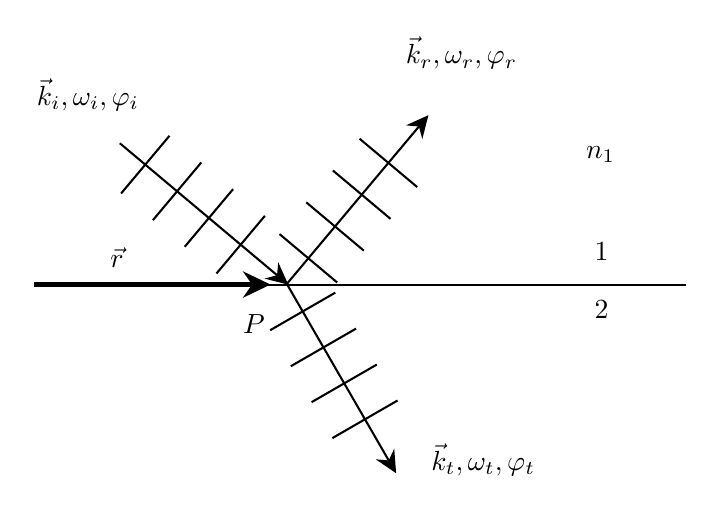
\begin{tikzpicture}[x=0.75pt,y=0.75pt,yscale=-1,xscale=1]
	%uncomment if require: \path (0,300); %set diagram left start at 0, and has height of 300

	%Straight Lines [id:da6183005433500193] 
	\draw    (164,167) -- (478,167) ;
	%Straight Lines [id:da22946316926380184] 
	\draw    (205.4,98.93) -- (284.3,165.14) ;
	\draw [shift={(286.6,167.07)}, rotate = 220] [fill={rgb, 255:red, 0; green, 0; blue, 0 }  ][line width=0.08]  [draw opacity=0] (10.72,-5.15) -- (0,0) -- (10.72,5.15) -- (7.12,0) -- cycle    ;
	%Straight Lines [id:da5066543042959124] 
	\draw    (275.27,133.9) -- (251.97,161.67) ;
	%Straight Lines [id:da00843700446911022] 
	\draw    (259.95,121.04) -- (236.65,148.81) ;
	%Straight Lines [id:da4219182653439604] 
	\draw    (244.63,108.19) -- (221.33,135.96) ;
	%Straight Lines [id:da7662075357732401] 
	\draw    (229.31,95.33) -- (206.01,123.1) ;

	%Straight Lines [id:da8746531724314954] 
	\draw    (285.93,166.6) -- (352.14,87.7) ;
	\draw [shift={(354.07,85.4)}, rotate = 490] [fill={rgb, 255:red, 0; green, 0; blue, 0 }  ][line width=0.08]  [draw opacity=0] (10.72,-5.15) -- (0,0) -- (10.72,5.15) -- (7.12,0) -- cycle    ;
	%Straight Lines [id:da9060241990807703] 
	\draw    (320.9,96.73) -- (348.67,120.03) ;
	%Straight Lines [id:da19712746629119682] 
	\draw    (308.04,112.05) -- (335.81,135.35) ;
	%Straight Lines [id:da7849526542504699] 
	\draw    (295.19,127.37) -- (322.96,150.67) ;
	%Straight Lines [id:da9233816968746384] 
	\draw    (282.33,142.69) -- (310.1,165.99) ;

	%Straight Lines [id:da5011592586326945] 
	\draw    (285.5,166.1) -- (337,255.3) ;
	\draw [shift={(338.5,257.9)}, rotate = 240] [fill={rgb, 255:red, 0; green, 0; blue, 0 }  ][line width=0.08]  [draw opacity=0] (10.72,-5.15) -- (0,0) -- (10.72,5.15) -- (7.12,0) -- cycle    ;
	%Straight Lines [id:da27638160120125854] 
	\draw    (339.2,222.86) -- (307.8,240.98) ;
	%Straight Lines [id:da6707584174541343] 
	\draw    (329.2,205.54) -- (297.8,223.66) ;
	%Straight Lines [id:da0469208813543982] 
	\draw    (319.2,188.22) -- (287.8,206.34) ;
	%Straight Lines [id:da38473496110325756] 
	\draw    (309.2,170.89) -- (277.8,189.02) ;

	%Straight Lines [id:da20096840221456458] 
	\draw [line width=1.5]    (164,167) -- (274,167) ;
	\draw [shift={(278,167)}, rotate = 180] [fill={rgb, 255:red, 0; green, 0; blue, 0 }  ][line width=0.08]  [draw opacity=0] (13.4,-6.43) -- (0,0) -- (13.4,6.44) -- (8.9,0) -- cycle    ;

	% Text Node
	\draw (270,186) node    {$P$};
	% Text Node
	\draw (204,154) node    {$\vec{r}$};
	% Text Node
	\draw (437.5,151) node    {$1$};
	% Text Node
	\draw (437.5,179) node    {$2$};
	% Text Node
	\draw (437,104.5) node    {$n_{1}$};
	% Text Node
	\draw (190,75.5) node    {$\vec{k}_{i} ,\omega _{i} ,\varphi _{i}$};
	% Text Node
	\draw (370,55.5) node    {$\vec{k}_{r} ,\omega _{r} ,\varphi _{r}$};
	% Text Node
	\draw (380.5,251.5) node    {$\vec{k}_{t} ,\omega _{t} ,\varphi _{t}$};

	\end{tikzpicture}
\end{figure}
\FloatBarrier

Nel momento in cui ciò accade, risulterà emergere un'\textbf{onda riflessa}. Essa sarà piana se la superficie è piana ma potrebbe avere una fase e un'ampiezza da determinare. Generalmente una porzione dell'onda incidente verrà anche trasmessa attraverso la superficie di separazione e propagherà. Quest'onda viene anche detta \textbf{onda trasmessa} o rifratta. Vogliamo determinare il legame fra queste tre onde.

Possiamo utilizzare le condizioni al contorno prima citate.
È necessario, perché questo siano rispettate, che gli argomenti dei seni delle sinusoidi siano gli stessi. Altrimenti non potremmo avere uguaglianza fra le componenti tangenti e normali dei vari campi. Si avrà allora che:

\[
	\vec{k}_i\cdot \vec{r} -\omega_it+\varphi_i = \vec{k}_r\cdot \vec{r} -\omega_rt+\varphi_r = \vec{k}_t\cdot \vec{r} -\omega_tt+\varphi_t
\]

Osserviamo che se poniamo $t=0$ e $r=0$ (scegliamo un certo istante e una certa posizione particolare), la relazione si semplifica:

\[
	\varphi_i = \varphi_r = \varphi_t
\]

Quindi di sicuro le tre fasi si eguagliano. Possiamo porre $\varphi=0$, cambiando così l'origine dei tempi, e portare tutte e tre le fasi a zero.
Se poniamo solo $r=0$, abbiamo:

\[
	-\omega_it = -\omega_rt = -\omega_tt
\]

Quindi anche le onde trasmesse e riflesse hanno la stessa frequenza. Parleremo d'ora in poi di $\omega$. A questo punto, rimane la relazione:

\begin{equation}
	\vec{k}_i\cdot \vec{r} = \vec{k}_r\cdot \vec{r} = \vec{k}_t\cdot \vec{r}
	\label{eq:uguaglianzaVetOnda}
\end{equation}

Scegliamo le coordinate in modo che la superficie di ha separazione coincida con il piano $xy$, su cui pertanto si trovano l'origine e il punto $P$ di incidenza. Inoltre l'asse $x$ è ortogonale al piano di incidenza individuato da $\vec{k}_i$ e da $\vec{k}_r$. Quindi $\vec{k}$ non ha componenti rispetto a tale variabile.

\begin{figure}[htpb]
	\centering

	\tikzset{every picture/.style={line width=0.75pt}} %set default line width to 0.75pt        

	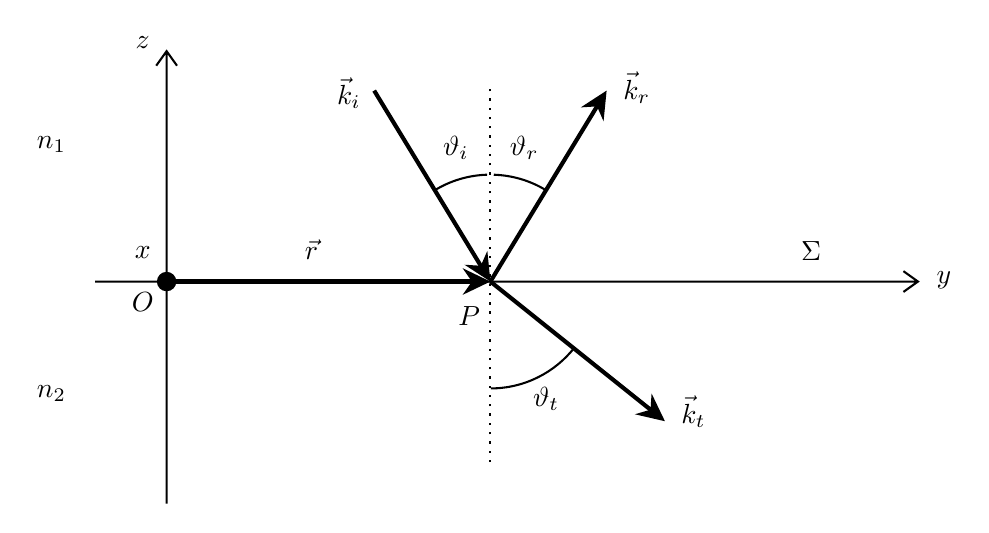
\begin{tikzpicture}[x=0.75pt,y=0.75pt,yscale=-1,xscale=1]
	%uncomment if require: \path (0,300); %set diagram left start at 0, and has height of 300

	%Shape: Axis 2D [id:dp43043438928604094] 
	\draw  (143,155) -- (539.5,155)(177.5,44) -- (177.5,262) (532.5,150) -- (539.5,155) -- (532.5,160) (172.5,51) -- (177.5,44) -- (182.5,51)  ;
	%Straight Lines [id:da6171096901926401] 
	\draw [line width=1.5]    (177.5,155) -- (329.5,155) ;
	\draw [shift={(333.5,155)}, rotate = 180] [fill={rgb, 255:red, 0; green, 0; blue, 0 }  ][line width=0.08]  [draw opacity=0] (13.4,-6.43) -- (0,0) -- (13.4,6.44) -- (8.9,0) -- cycle    ;
	%Straight Lines [id:da7950107605009162] 
	\draw [line width=1.5]    (277.5,63) -- (331.42,151.58) ;
	\draw [shift={(333.5,155)}, rotate = 238.67000000000002] [fill={rgb, 255:red, 0; green, 0; blue, 0 }  ][line width=0.08]  [draw opacity=0] (13.4,-6.43) -- (0,0) -- (13.4,6.44) -- (8.9,0) -- cycle    ;
	%Straight Lines [id:da4358193570786466] 
	\draw [line width=1.5]    (387.42,66.42) -- (333.5,155) ;
	\draw [shift={(389.5,63)}, rotate = 121.33] [fill={rgb, 255:red, 0; green, 0; blue, 0 }  ][line width=0.08]  [draw opacity=0] (13.4,-6.43) -- (0,0) -- (13.4,6.44) -- (8.9,0) -- cycle    ;
	%Straight Lines [id:da06331109301956106] 
	\draw [line width=1.5]    (333.5,155) -- (414.47,219.8) ;
	\draw [shift={(417.59,222.3)}, rotate = 218.67000000000002] [fill={rgb, 255:red, 0; green, 0; blue, 0 }  ][line width=0.08]  [draw opacity=0] (13.4,-6.43) -- (0,0) -- (13.4,6.44) -- (8.9,0) -- cycle    ;
	%Straight Lines [id:da2398676595359941] 
	\draw [line width=0.75]  [dash pattern={on 0.84pt off 2.51pt}]  (333.5,242) -- (333.5,60) ;
	%Shape: Circle [id:dp75582930196853] 
	\draw  [fill={rgb, 255:red, 0; green, 0; blue, 0 }  ,fill opacity=1 ] (173.33,155) .. controls (173.33,152.7) and (175.2,150.83) .. (177.5,150.83) .. controls (179.8,150.83) and (181.67,152.7) .. (181.67,155) .. controls (181.67,157.3) and (179.8,159.17) .. (177.5,159.17) .. controls (175.2,159.17) and (173.33,157.3) .. (173.33,155) -- cycle ;
	%Shape: Arc [id:dp8841166469092541] 
	\draw  [draw opacity=0] (306.43,111.18) .. controls (313.88,106.57) and (322.59,103.81) .. (331.92,103.52) -- (333.5,155) -- cycle ; \draw   (306.43,111.18) .. controls (313.88,106.57) and (322.59,103.81) .. (331.92,103.52) ;
	%Shape: Arc [id:dp5001740494755782] 
	\draw  [draw opacity=0] (335.13,103.53) .. controls (344.19,103.81) and (352.67,106.43) .. (359.97,110.81) -- (333.5,155) -- cycle ; \draw   (335.13,103.53) .. controls (344.19,103.81) and (352.67,106.43) .. (359.97,110.81) ;
	%Shape: Arc [id:dp2155363034717026] 
	\draw  [draw opacity=0] (373.98,186.84) .. controls (364.6,198.75) and (350.08,206.42) .. (333.77,206.5) -- (333.5,155) -- cycle ; \draw   (373.98,186.84) .. controls (364.6,198.75) and (350.08,206.42) .. (333.77,206.5) ;

	% Text Node
	\draw (122,89) node    {$n_{1}$};
	% Text Node
	\draw (122,209) node    {$n_{2}$};
	% Text Node
	\draw (166,165) node    {$O$};
	% Text Node
	\draw (166,40) node    {$z$};
	% Text Node
	\draw (247.33,139.67) node    {$\vec{r}$};
	% Text Node
	\draw (323.33,171.67) node    {$P$};
	% Text Node
	\draw (265.33,64.33) node    {$\vec{k}_{i}$};
	% Text Node
	\draw (404,61.67) node    {$\vec{k}_{r}$};
	% Text Node
	\draw (431.33,217.67) node    {$\vec{k}_{t}$};
	% Text Node
	\draw (166,141) node    {$x$};
	% Text Node
	\draw (552,154.33) node    {$y$};
	% Text Node
	\draw (488,140.33) node    {$\Sigma $};
	% Text Node
	\draw (316.83,90.67) node    {$\vartheta _{i}$};
	% Text Node
	\draw (349.83,90.67) node    {$\vartheta _{r}$};
	% Text Node
	\draw (360.33,211.67) node    {$\vartheta _{t}$};

	\end{tikzpicture}
\end{figure}
\FloatBarrier

\begin{align*}
	\vec{k}_i &= \underbrace{k_{ix}}_{=0} \vec{u}_x + k_{iy} \vec{u}_y + k_{iz} \vec{u}_z \\
	\vec{k}_i\cdot \vec{r}  &= (k_{iy} \vec{u}_y + k_{iz} \vec{u}_z)\cdot \vec{r} \tag*{moltiplico per $\vec{r}$}\\
	\vec{k}_i\cdot \vec{r}  &= (k_{iy} \vec{u}_y + k_{iz} \vec{u}_z)\cdot (x\vec{u}_x+y\vec{u}_y) \tag*{$\vec{r}$ sta su $xy$}\\
	\vec{k}_i\cdot \vec{r}  &= k_{iy} \,y \\
	\vec{k}_r\cdot \vec{r} = \vec{k}_t\cdot \vec{r}  &= k_{iy} \,y
\end{align*}

Queste uguaglianza deve valere per qualsiasi valore di $x$ e di $y$, cioè per qualsiasi posizione di $P$ sul piano, quindi deve essere:

\[
	k_{rx} = 0 \qquad k_{tx} = 0 \qquad k_{rz} = 0 \qquad k_{tz} = 0
\]

Dal momento che anche $k_t$ e $k_r$ hanno la componente in $x$ nulla, si deduce che giacciono sul piano di incidenza. Si enuncia pertanto la \textbf{prima legge della riflessione e della rifrazione}:\\
\emph{Le direzioni di propagazione dell'onda incidente, riflessa e rifratta giacciono nel piano di incidenza, individuato dalla direzione di incidenza e dalla normale alla superficie di separazione nel punto di incidenza.}

\begin{itemize}
	\item Chiameremo $\vartheta_i$ l'angolo che il vettore dell'onda incidente forma con la normale alla superficie. Esso prende il nome di \textbf{angolo di incidenza}.
	\item Chiamiamo \textbf{angolo di riflessione} $\vartheta_r$ quello che $\vec{k}_r$ forma con la normale.
	\item Analogamente chiameremo \textbf{angolo di trasmissione} o di rifrazione $\vartheta_t$ quello che $k_t$ forma con la normale.
\end{itemize}

La componente lungo l'asse $y$ di $\vec{k}_i$ è pari a:

\[
	k_{iy} = |\vec{k}_i |\sin \vartheta_i = \frac{\omega n_1}{c}\sin \vartheta_i
\]

A questo punto è semplice scrivere anche le altre componenti:

\begin{align*}
	k_{ry} &= |\vec{k}_r |\sin \vartheta_r = \frac{\omega n_1}{c}\sin \vartheta_r \\
	k_{ty} &= |\vec{k}_t |\sin \vartheta_t = \frac{\omega n_2}{c}\sin \vartheta_t \\
	k_{iy}&=k_{ry} \implies \frac{\omega n_1}{c}\sin \vartheta_i = \frac{\omega n_1}{c}\sin \vartheta_r \implies \boxed{\vartheta_i=\vartheta_r}\\
	k_{iy}&=k_{ty} \implies \frac{\omega n_1}{c}\sin \vartheta_i = \frac{\omega n_2}{c}\sin \vartheta_t \implies \boxed{n_1\sin  \vartheta_i=n_2\sin  \vartheta_r}\\
\end{align*}

Questo risultato è noto come \textbf{legge di Snell}.
Detto $n_2/n_1$ \emph{indice di rifrazione relativo del secondo mezzo rispetto al primo}, la legge di Snell viene enunciata dicendo:\\
\emph{Il rapporto tra il seno dell'angolo di incidenza e il seno dell'angolo di rifrazione è costante ed eguale all'indice di rifrazione relativo fra i due mezzi.}\\
La legge di Snell può anche essere utilizzata come definizione operativa dell'indice di rifrazione di una sostanza trasparente relativo ad un mezzo campione, ovvero dell'indice assoluto rispetto al vuoto. Per eseguire la misura, deve però essere possibile definire una superficie di separazione tra il mezzo in esame e il mezzo esterno con indice di rifrazione noto. Il metodo quindi non si applica ai gas.

Nella legge $\vartheta_i=\vartheta_r  $ non compare invece alcuna caratteristica del mezzo in cui si propaga l'onda incidente e l'onda riflessa. L'angolo di riflessione è sempre lo stesso, eguale all'angolo di incidenza, qualunque sia la lunghezza d'onda della luce incidente e non c'è dispersione.

La legge di Snell ci permette di studiare due casi in particolare.

\begin{itemize}
	\item Caso $n_1<n_2$. Qualunque sia l'angolo di incidenza, c'è sempre soluzione per la legge di Snell, quindi si trova sempre un corrispondente angolo di trasmissione. Infatti:
	\[
		\forall \vartheta_i\qquad \sin \vartheta_t= \frac{n_1}{n_2}\sin \vartheta_i \le 1
	\]
	\begin{figure}[htpb]
		\centering
		

		\tikzset{every picture/.style={line width=0.75pt}} %set default line width to 0.75pt        

		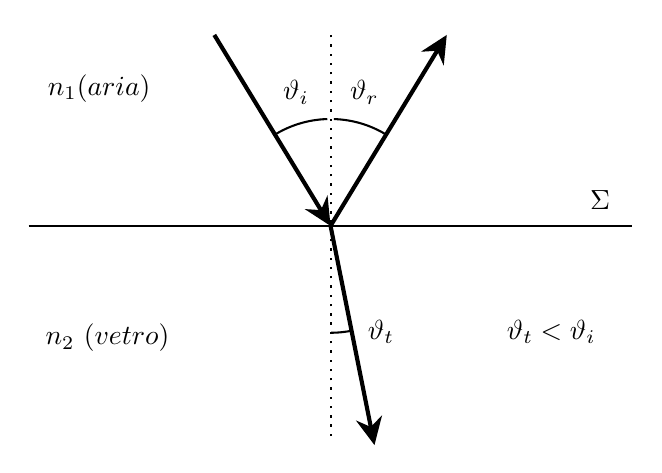
\begin{tikzpicture}[x=0.75pt,y=0.75pt,yscale=-1,xscale=1]
		%uncomment if require: \path (0,300); %set diagram left start at 0, and has height of 300

		%Straight Lines [id:da5050294782052775] 
		\draw [line width=0.75]    (167.08,154) -- (457.92,154) ;
		%Straight Lines [id:da8251861314221638] 
		\draw [line width=1.5]    (256.5,62) -- (310.42,150.58) ;
		\draw [shift={(312.5,154)}, rotate = 238.67000000000002] [fill={rgb, 255:red, 0; green, 0; blue, 0 }  ][line width=0.08]  [draw opacity=0] (13.4,-6.43) -- (0,0) -- (13.4,6.44) -- (8.9,0) -- cycle    ;
		%Straight Lines [id:da4739059636586811] 
		\draw [line width=1.5]    (366.42,65.42) -- (312.5,154) ;
		\draw [shift={(368.5,62)}, rotate = 121.33] [fill={rgb, 255:red, 0; green, 0; blue, 0 }  ][line width=0.08]  [draw opacity=0] (13.4,-6.43) -- (0,0) -- (13.4,6.44) -- (8.9,0) -- cycle    ;
		%Straight Lines [id:da44077768680661067] 
		\draw [line width=1.5]    (312.5,154) -- (332.87,255.68) ;
		\draw [shift={(333.66,259.6)}, rotate = 258.67] [fill={rgb, 255:red, 0; green, 0; blue, 0 }  ][line width=0.08]  [draw opacity=0] (13.4,-6.43) -- (0,0) -- (13.4,6.44) -- (8.9,0) -- cycle    ;
		%Straight Lines [id:da7486337079341854] 
		\draw [line width=0.75]  [dash pattern={on 0.84pt off 2.51pt}]  (312.5,255.25) -- (312.5,59) ;
		%Shape: Arc [id:dp3100987369844985] 
		\draw  [draw opacity=0] (285.43,110.18) .. controls (292.88,105.57) and (301.59,102.81) .. (310.92,102.52) -- (312.5,154) -- cycle ; \draw   (285.43,110.18) .. controls (292.88,105.57) and (301.59,102.81) .. (310.92,102.52) ;
		%Shape: Arc [id:dp6634686778117325] 
		\draw  [draw opacity=0] (314.13,102.53) .. controls (323.19,102.81) and (331.67,105.43) .. (338.97,109.81) -- (312.5,154) -- cycle ; \draw   (314.13,102.53) .. controls (323.19,102.81) and (331.67,105.43) .. (338.97,109.81) ;
		%Shape: Arc [id:dp36248656848360494] 
		\draw  [draw opacity=0] (322.77,204.48) .. controls (319.54,205.13) and (316.19,205.48) .. (312.77,205.5) -- (312.5,154) -- cycle ; \draw   (322.77,204.48) .. controls (319.54,205.13) and (316.19,205.48) .. (312.77,205.5) ;

		% Text Node
		\draw (201,88) node    {$n_{1}\text{ (aria)}$};
		% Text Node
		\draw (205,208) node    {$n_{2} \ \text{(vetro)}$};
		% Text Node
		\draw (442.33,141.33) node    {$\Sigma $};
		% Text Node
		\draw (295.83,89.67) node    {$\vartheta _{i}$};
		% Text Node
		\draw (328.83,89.67) node    {$\vartheta _{r}$};
		% Text Node
		\draw (336.83,205.17) node    {$\vartheta _{t}$};
		% Text Node
		\draw (418.83,205.17) node    {$\vartheta _{t} < \vartheta _{i}$};

		\end{tikzpicture}
	\end{figure}
	\FloatBarrier

	\item Caso $n_2<n_1$. All'aumentare dell'angolo di incidenza, l'onda trasmessa arriverà a propagare lungo la superficie di separazione per poi essere totalmente riflessa. Il rapporto $n_1/n_2$ infatti è maggiore di $1$, quindi il seno dell'angolo trasmesso non potrà essere definito per qualsiasi ampiezza di $ \vartheta_i  $.
	\[
		\sin \vartheta_t = \frac{n_1}{n_2}\sin \vartheta_i
	\]
	Quell'angolo per il quale $\sin \vartheta_t $ è pari a $1$ è detto \textbf{angolo limite}. L'onda viene subito deflessa. Per trovarlo basta invertire l'equazione, trovando:
	\[
		\vartheta_i = \arcsin \left( \frac{n_2}{n_1} \right)
	\]
	\begin{figure}[htpb]
		\centering
		

		\tikzset{every picture/.style={line width=0.75pt}} %set default line width to 0.75pt        

		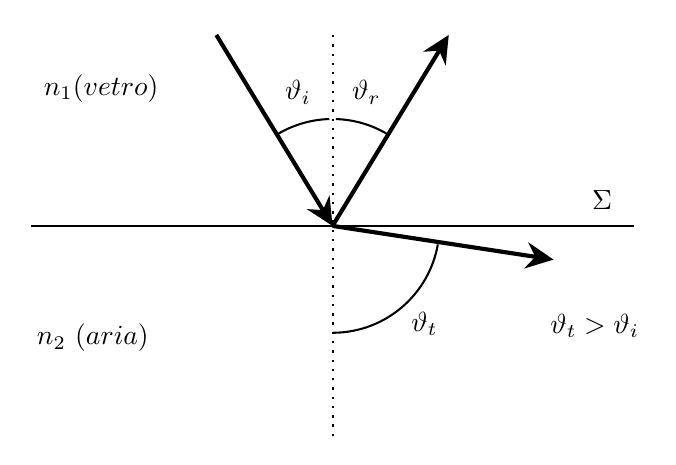
\begin{tikzpicture}[x=0.75pt,y=0.75pt,yscale=-1,xscale=1]
		%uncomment if require: \path (0,300); %set diagram left start at 0, and has height of 300

		%Straight Lines [id:da965119002350822] 
		\draw [line width=0.75]    (167.08,154) -- (457.92,154) ;
		%Straight Lines [id:da41123154558130426] 
		\draw [line width=1.5]    (256.5,62) -- (310.42,150.58) ;
		\draw [shift={(312.5,154)}, rotate = 238.67000000000002] [fill={rgb, 255:red, 0; green, 0; blue, 0 }  ][line width=0.08]  [draw opacity=0] (13.4,-6.43) -- (0,0) -- (13.4,6.44) -- (8.9,0) -- cycle    ;
		%Straight Lines [id:da2239839616290593] 
		\draw [line width=1.5]    (366.42,65.42) -- (312.5,154) ;
		\draw [shift={(368.5,62)}, rotate = 121.33] [fill={rgb, 255:red, 0; green, 0; blue, 0 }  ][line width=0.08]  [draw opacity=0] (13.4,-6.43) -- (0,0) -- (13.4,6.44) -- (8.9,0) -- cycle    ;
		%Straight Lines [id:da8708148668464029] 
		\draw [line width=1.5]    (312.5,154) -- (415.02,169.63) ;
		\draw [shift={(418.97,170.24)}, rotate = 188.67] [fill={rgb, 255:red, 0; green, 0; blue, 0 }  ][line width=0.08]  [draw opacity=0] (13.4,-6.43) -- (0,0) -- (13.4,6.44) -- (8.9,0) -- cycle    ;
		%Straight Lines [id:da37791866391045437] 
		\draw [line width=0.75]  [dash pattern={on 0.84pt off 2.51pt}]  (312.5,255.25) -- (312.5,59) ;
		%Shape: Arc [id:dp2694839214350737] 
		\draw  [draw opacity=0] (285.43,110.18) .. controls (292.88,105.57) and (301.59,102.81) .. (310.92,102.52) -- (312.5,154) -- cycle ; \draw   (285.43,110.18) .. controls (292.88,105.57) and (301.59,102.81) .. (310.92,102.52) ;
		%Shape: Arc [id:dp3463452444005113] 
		\draw  [draw opacity=0] (314.13,102.53) .. controls (323.19,102.81) and (331.67,105.43) .. (338.97,109.81) -- (312.5,154) -- cycle ; \draw   (314.13,102.53) .. controls (323.19,102.81) and (331.67,105.43) .. (338.97,109.81) ;
		%Shape: Arc [id:dp5103197837937474] 
		\draw  [draw opacity=0] (363.23,162.92) .. controls (359.02,187.02) and (338.05,205.37) .. (312.77,205.5) -- (312.5,154) -- cycle ; \draw   (363.23,162.92) .. controls (359.02,187.02) and (338.05,205.37) .. (312.77,205.5) ;

		% Text Node
		\draw (201,88) node    {$n_{1}\text{ (vetro)}$};
		% Text Node
		\draw (197,208) node    {$n_{2} \ \text{(aria)}$};
		% Text Node
		\draw (442.33,141.33) node    {$\Sigma $};
		% Text Node
		\draw (295.83,89.67) node    {$\vartheta _{i}$};
		% Text Node
		\draw (328.83,89.67) node    {$\vartheta _{r}$};
		% Text Node
		\draw (356.83,201.17) node    {$\vartheta _{t}$};
		% Text Node
		\draw (438.83,202.17) node    {$\vartheta _{t}  >\vartheta _{i}$};

		\end{tikzpicture}
	\end{figure}
	\FloatBarrier

\end{itemize}

Aumentando l'angolo l'incidenza oltre l'angolo limite, non ci sarà più trasmissione. Si parla di un fenomeno noto come \textbf{riflessione totale}, tutta l'onda incidente viene riflessa. Questa proprietà viene altamente sfruttata nelle \emph{fibre ottiche}. Una fibra ottica è un cilindro di vetro di indice di rifrazione maggiore rispetto al mezzo in cui è immerso. La luce che penetra nel cilindro attraverso una base incide sulle pareti laterali formando un angolo superiore all'angolo limite e viene riflessa totalmente molte volte, senza apprezzabili perdite, fino ad uscire dall'altra base. Questa tecnica è usata in medicina per l'osservazione di organi interni (endoscopia): con un fascio di fibre si convoglia la luce di una sorgente esterna sulla parte da osservare e con un altro fascio si riceve la luce diffusa dalla parte illuminata. Un'altra applicazione importante e in rapido sviluppo si ha nel campo delle telecomunicazioni.

\section{Dispersione della luce in un mezzo trasparente}

Quando nel fascio incidente sono contenute più lunghezze d'onda, ad un dato angolo di incidenza corrispondono più angoli di rifrazione. L'indice di rifrazione infatti dipende dalla frequenza e diminuisce al crescere della lunghezza d'onda. Se ci riferiamo a onde elettromagnetiche dello spettro visibile, in tutti i materiali si trova che $n_{\text{rosso}} < n_{\text{verde}} < n_{\text{blu}}$.
Se ad esempio un sottile fascio di luce bianca, che contiene tutte le lunghezze d'onda visibili, incide su una lastra di vetro, la luce riflessa è ancora bianca mentre il fascio trasmesso nel vetro è composto da una serie di raggi di colore diversi, ognuno con diverso angolo di rifrazione. È questo aspetto del fenomeno che ha dato origine al termine \textbf{dispersione della luce}.
La dispersione della luce spiega anche il fenomeno degli arcobaleni. La luce del sole viene trasmessa dalle gocce d'acqua, e i colori appaiono quindi separati.

\section{Intensità delle onde elettromagnetiche riflesse e rifratte. Formule di Fresnel}

Le relazioni tra le ampiezze si ricavano dalle equazioni di Maxwell, precisamente dalle condizioni di continuità dei campi.

\subsection{Caso trasversale magnetico (TM)}

In figura è indicata la situazione in cui il campo elettrico incidente è polarizzato n rettilinearmente nel piano $\pi$ di incidenza. Il campo $\vec{B}$ inoltre è perpendicolare al piano del foglio ed è continuo nel passaggio attraverso la superficie in quanto assumiamo trascurabili le proprietà magnetiche dei dielettrici.

\begin{figure}[htpb]
	\centering

	\tikzset{every picture/.style={line width=0.75pt}} %set default line width to 0.75pt        

	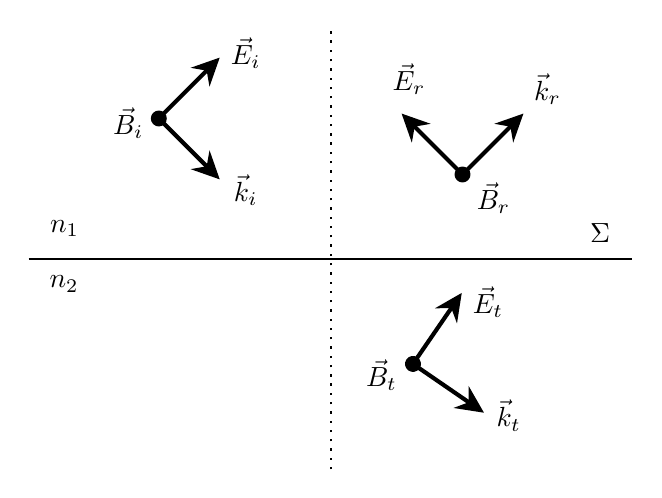
\begin{tikzpicture}[x=0.75pt,y=0.75pt,yscale=-1,xscale=1]
	%uncomment if require: \path (0,300); %set diagram left start at 0, and has height of 300

	%Straight Lines [id:da2090760346759728] 
	\draw [line width=0.75]    (175.08,159) -- (465.92,159) ;
	%Straight Lines [id:da019521017012416708] 
	\draw [line width=1.5]    (237.76,91.25) -- (264.28,117.77) ;
	\draw [shift={(267.11,120.59)}, rotate = 225] [fill={rgb, 255:red, 0; green, 0; blue, 0 }  ][line width=0.08]  [draw opacity=0] (13.4,-6.43) -- (0,0) -- (13.4,6.44) -- (8.9,0) -- cycle    ;
	%Straight Lines [id:da8473806581412822] 
	\draw [line width=1.5]    (237.76,91.25) -- (264.28,64.73) ;
	\draw [shift={(267.11,61.91)}, rotate = 495] [fill={rgb, 255:red, 0; green, 0; blue, 0 }  ][line width=0.08]  [draw opacity=0] (13.4,-6.43) -- (0,0) -- (13.4,6.44) -- (8.9,0) -- cycle    ;
	%Shape: Circle [id:dp2638401536274628] 
	\draw  [fill={rgb, 255:red, 0; green, 0; blue, 0 }  ,fill opacity=1 ] (235.41,88.89) .. controls (236.71,87.59) and (238.82,87.59) .. (240.12,88.89) .. controls (241.42,90.19) and (241.42,92.31) .. (240.12,93.61) .. controls (238.82,94.91) and (236.71,94.91) .. (235.41,93.61) .. controls (234.1,92.31) and (234.1,90.19) .. (235.41,88.89) -- cycle ;

	%Straight Lines [id:da7803022354972504] 
	\draw [line width=0.75]  [dash pattern={on 0.84pt off 2.51pt}]  (320.5,260.25) -- (320.5,48) ;
	%Straight Lines [id:da7670188340524602] 
	\draw [line width=1.5]    (384.08,118.24) -- (410.6,91.72) ;
	\draw [shift={(413.43,88.89)}, rotate = 495] [fill={rgb, 255:red, 0; green, 0; blue, 0 }  ][line width=0.08]  [draw opacity=0] (13.4,-6.43) -- (0,0) -- (13.4,6.44) -- (8.9,0) -- cycle    ;
	%Straight Lines [id:da8684392720931324] 
	\draw [line width=1.5]    (384.08,118.24) -- (357.57,91.72) ;
	\draw [shift={(354.74,88.89)}, rotate = 405] [fill={rgb, 255:red, 0; green, 0; blue, 0 }  ][line width=0.08]  [draw opacity=0] (13.4,-6.43) -- (0,0) -- (13.4,6.44) -- (8.9,0) -- cycle    ;
	%Shape: Circle [id:dp6351258422342285] 
	\draw  [fill={rgb, 255:red, 0; green, 0; blue, 0 }  ,fill opacity=1 ] (381.73,120.59) .. controls (380.42,119.29) and (380.42,117.18) .. (381.73,115.88) .. controls (383.03,114.58) and (385.14,114.58) .. (386.44,115.88) .. controls (387.74,117.18) and (387.74,119.29) .. (386.44,120.59) .. controls (385.14,121.9) and (383.03,121.9) .. (381.73,120.59) -- cycle ;

	%Straight Lines [id:da860631649047952] 
	\draw [line width=1.5]    (360.21,209.51) -- (391.12,230.74) ;
	\draw [shift={(394.42,233.01)}, rotate = 214.49] [fill={rgb, 255:red, 0; green, 0; blue, 0 }  ][line width=0.08]  [draw opacity=0] (13.4,-6.43) -- (0,0) -- (13.4,6.44) -- (8.9,0) -- cycle    ;
	%Straight Lines [id:da735762826157579] 
	\draw [line width=1.5]    (360.21,209.51) -- (381.45,178.6) ;
	\draw [shift={(383.71,175.3)}, rotate = 484.49] [fill={rgb, 255:red, 0; green, 0; blue, 0 }  ][line width=0.08]  [draw opacity=0] (13.4,-6.43) -- (0,0) -- (13.4,6.44) -- (8.9,0) -- cycle    ;
	%Shape: Circle [id:dp8501408964699348] 
	\draw  [fill={rgb, 255:red, 0; green, 0; blue, 0 }  ,fill opacity=1 ] (357.47,207.62) .. controls (358.51,206.1) and (360.59,205.72) .. (362.1,206.76) .. controls (363.62,207.8) and (364,209.88) .. (362.96,211.39) .. controls (361.92,212.91) and (359.84,213.3) .. (358.33,212.25) .. controls (356.81,211.21) and (356.42,209.14) .. (357.47,207.62) -- cycle ;

	% Text Node
	\draw (192.33,144.33) node    {$n_{1}$};
	% Text Node
	\draw (194.33,171) node    {$n_{2} \ $};
	% Text Node
	\draw (450.33,146.33) node    {$\Sigma $};
	% Text Node
	\draw (279.67,125.67) node    {$\vec{k}_{i}$};
	% Text Node
	\draw (279.67,59.67) node    {$\vec{E}_{i}$};
	% Text Node
	\draw (223,93.67) node    {$\vec{B}_{i}$};
	% Text Node
	\draw (425,77) node    {$\vec{k}_{r}$};
	% Text Node
	\draw (358.33,72.33) node    {$\vec{E}_{r}$};
	% Text Node
	\draw (399,129.67) node    {$\vec{B}_{r}$};
	% Text Node
	\draw (345,215) node    {$\vec{B}_{t}$};
	% Text Node
	\draw (396.33,179.67) node    {$\vec{E}_{t}$};
	% Text Node
	\draw (406.33,234.33) node    {$\vec{k}_{t}$};

	\end{tikzpicture}
\end{figure}
\FloatBarrier

\[
	\vec{B}_i + \vec{B}_r = \vec{B}_t
\]

Affinché questa uguaglianza sia soddisfatta, $\vec{B}_r$ e $\vec{B}_t$ devono anche essi essere ortogonali al piano di incidenza come $\vec{B}_i$. Quindi il campo elettrico riflesso e rifratto sono anche essi polarizzati nel piano di incidenza. Sapendo che:

\[
	B=\frac{E}{v}=\frac{nE}{c}
\]

Possiamo scrivere:

\[
	\frac{n_1E_i}{c} + \frac{n_1E_r}{c} = \frac{n_2E_t}{c}
\]

Inoltre, dal momento che la componente normale del campo elettrico si conserva (condizioni al contorno):

\[
	E_i\cos \vartheta_i - E_r\cos \vartheta_r = E_t\cos \vartheta_t
\]

Abbiamo così un sistema di due equazioni che ci permette di arrivare a due risultati:

\begin{gather*}
	\left\{ \begin{array}{l}
	 	\frac{n_1E_i}{c} + \frac{n_1E_r}{c} = \frac{n_2E_t}{c} \\
		E_i\cos \vartheta_i - E_r\cos \vartheta_r = E_t\cos \vartheta_t
	\end{array} \right.\\\\
	\boxed{\frac{E_r}{E_i} = \frac{n_2\cos \vartheta_i-n_1\cos \vartheta_t}{n_2\cos \vartheta_i + n_1\cos \vartheta_t}}\qquad
	\boxed{\frac{E_t}{E_i} = \frac{2n_1\cos \vartheta_i}{n_1\cos \vartheta_t + n_2\cos \vartheta_i}}
\end{gather*}

Queste sono note come \textbf{formule di Fresnel} nel piano di incidenza $\pi$. Esse permettono di calcolare a partire dall'ampiezza incidente le ampiezze riflesse e rifratte: dipendono soltanto dall'angolo di incidenza e dall'angolo di rifrazione.

\subsection{Caso trasversale elettrico (TE)}

Si tratta di un caso complementare in cui si invertono i ruoli dei due campi. $\vec{E}$ è polarizzato rettilinearmente ed è ortogonale al piano di incidenza $\pi$. Anche in questo caso si dimostra che i campi elettrici riflesso e rifratto mantengono la polarizzazione del campo elettrico incidente, per cui i campi magnetici stanno tutti su $\pi$.

\begin{figure}[htpb]
	\centering

	\tikzset{every picture/.style={line width=0.75pt}} %set default line width to 0.75pt        

	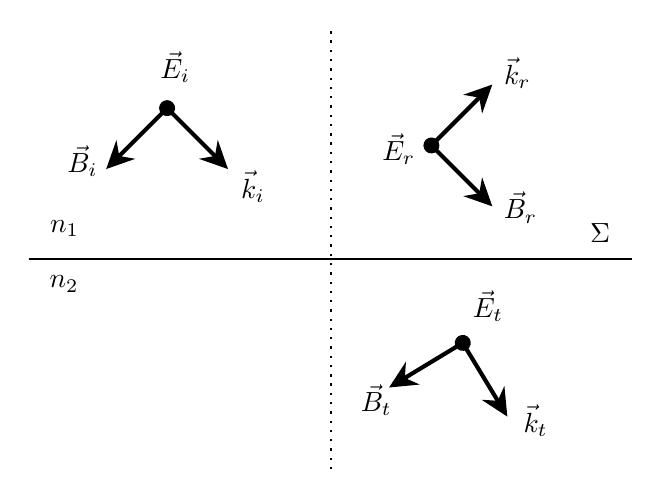
\begin{tikzpicture}[x=0.75pt,y=0.75pt,yscale=-1,xscale=1]
	%uncomment if require: \path (0,300); %set diagram left start at 0, and has height of 300

	%Straight Lines [id:da146620167581893] 
	\draw [line width=0.75]    (188.08,170) -- (478.92,170) ;
	%Straight Lines [id:da48568077110951213] 
	\draw [line width=1.5]    (254.75,97.26) -- (228.23,123.78) ;
	\draw [shift={(225.41,126.61)}, rotate = 315] [fill={rgb, 255:red, 0; green, 0; blue, 0 }  ][line width=0.08]  [draw opacity=0] (13.4,-6.43) -- (0,0) -- (13.4,6.44) -- (8.9,0) -- cycle    ;
	%Straight Lines [id:da48687204867088085] 
	\draw [line width=1.5]    (254.75,97.26) -- (281.27,123.78) ;
	\draw [shift={(284.09,126.61)}, rotate = 225] [fill={rgb, 255:red, 0; green, 0; blue, 0 }  ][line width=0.08]  [draw opacity=0] (13.4,-6.43) -- (0,0) -- (13.4,6.44) -- (8.9,0) -- cycle    ;
	%Shape: Circle [id:dp25299218306132554] 
	\draw  [fill={rgb, 255:red, 0; green, 0; blue, 0 }  ,fill opacity=1 ] (257.11,94.91) .. controls (258.41,96.21) and (258.41,98.32) .. (257.11,99.62) .. controls (255.81,100.92) and (253.69,100.92) .. (252.39,99.62) .. controls (251.09,98.32) and (251.09,96.21) .. (252.39,94.91) .. controls (253.69,93.6) and (255.81,93.6) .. (257.11,94.91) -- cycle ;

	%Straight Lines [id:da8386406799955135] 
	\draw [line width=0.75]  [dash pattern={on 0.84pt off 2.51pt}]  (333.5,271.25) -- (333.5,59) ;
	%Straight Lines [id:da70976718398795] 
	\draw [line width=1.5]    (382.1,115.25) -- (408.61,141.77) ;
	\draw [shift={(411.44,144.59)}, rotate = 225] [fill={rgb, 255:red, 0; green, 0; blue, 0 }  ][line width=0.08]  [draw opacity=0] (13.4,-6.43) -- (0,0) -- (13.4,6.44) -- (8.9,0) -- cycle    ;
	%Straight Lines [id:da10798554149673545] 
	\draw [line width=1.5]    (382.1,115.25) -- (408.61,88.73) ;
	\draw [shift={(411.44,85.91)}, rotate = 495] [fill={rgb, 255:red, 0; green, 0; blue, 0 }  ][line width=0.08]  [draw opacity=0] (13.4,-6.43) -- (0,0) -- (13.4,6.44) -- (8.9,0) -- cycle    ;
	%Shape: Circle [id:dp29239224121168195] 
	\draw  [fill={rgb, 255:red, 0; green, 0; blue, 0 }  ,fill opacity=1 ] (379.74,112.89) .. controls (381.04,111.59) and (383.15,111.59) .. (384.45,112.89) .. controls (385.75,114.19) and (385.75,116.31) .. (384.45,117.61) .. controls (383.15,118.91) and (381.04,118.91) .. (379.74,117.61) .. controls (378.44,116.31) and (378.44,114.19) .. (379.74,112.89) -- cycle ;

	%Straight Lines [id:da25353547697892953] 
	\draw [line width=1.5]    (397.2,210.38) -- (365.11,229.79) ;
	\draw [shift={(361.69,231.86)}, rotate = 328.83000000000004] [fill={rgb, 255:red, 0; green, 0; blue, 0 }  ][line width=0.08]  [draw opacity=0] (13.4,-6.43) -- (0,0) -- (13.4,6.44) -- (8.9,0) -- cycle    ;
	%Straight Lines [id:da08542631169290593] 
	\draw [line width=1.5]    (397.2,210.38) -- (416.61,242.46) ;
	\draw [shift={(418.68,245.89)}, rotate = 238.82999999999998] [fill={rgb, 255:red, 0; green, 0; blue, 0 }  ][line width=0.08]  [draw opacity=0] (13.4,-6.43) -- (0,0) -- (13.4,6.44) -- (8.9,0) -- cycle    ;
	%Shape: Circle [id:dp18706324259343288] 
	\draw  [fill={rgb, 255:red, 0; green, 0; blue, 0 }  ,fill opacity=1 ] (400.05,208.65) .. controls (401.01,210.23) and (400.5,212.28) .. (398.93,213.23) .. controls (397.35,214.18) and (395.3,213.68) .. (394.35,212.1) .. controls (393.4,210.53) and (393.9,208.48) .. (395.48,207.53) .. controls (397.05,206.57) and (399.1,207.08) .. (400.05,208.65) -- cycle ;

	% Text Node
	\draw (205.33,155.33) node    {$n_{1}$};
	% Text Node
	\draw (207.33,182) node    {$n_{2} \ $};
	% Text Node
	\draw (463.33,157.33) node    {$\Sigma $};
	% Text Node
	\draw (296.17,135.17) node    {$\vec{k}_{i}$};
	% Text Node
	\draw (258.67,77.67) node    {$\vec{E}_{i}$};
	% Text Node
	\draw (214,122.67) node    {$\vec{B}_{i}$};
	% Text Node
	\draw (423.5,80.5) node    {$\vec{k}_{r}$};
	% Text Node
	\draw (366.33,116.83) node    {$\vec{E}_{r}$};
	% Text Node
	\draw (425,145.17) node    {$\vec{B}_{r}$};
	% Text Node
	\draw (355.5,238) node    {$\vec{B}_{t}$};
	% Text Node
	\draw (409.33,192.67) node    {$\vec{E}_{t}$};
	% Text Node
	\draw (432.33,247.83) node    {$\vec{k}_{t}$};

	\end{tikzpicture}
\end{figure}
\FloatBarrier

Procediamo in modo analogo al caso precedente:

\[
	\vec{B} =\mu_0 \vec{H} \implies \vec{H} = \frac{\vec{B}}{\mu_0} \qquad B = \frac{nE}{c}
\]

Per le condizioni al contorno:

\[
	\left\{ \begin{array}{l}
	 	-\frac{B_i}{\mu_0}\cos \vartheta_i + \frac{B_r}{\mu_0}\sin \vartheta_r = - \frac{B_t}{\mu_0}\cos \vartheta_t\\
	 	\vec{E}_i + \vec{E}_r = \vec{E}_t
	\end{array} \right.
\]

si trovano le equazioni di Fresnel nel piano ortogonale a quello di incidenza:

\[
	\boxed{\frac{E_r}{E_i} = \frac{n_1\cos \vartheta_i-n_2\cos \vartheta_t}{n_1\cos \vartheta_i + n_2\cos \vartheta_t}}\qquad
	\boxed{\frac{E_t}{E_i} = \frac{2n_1\cos \vartheta_i}{n_1\cos \vartheta_i + n_2\cos \vartheta_t}}
\]

Un aspetto interessante è che l'ampiezza dell'onda riflessa è diversa nei vari casi. Generalmente accade che se consideriamo una superficie di separazione fra l'aria e un mezzo di indice di rifrazione maggiore (ad esempio l'acqua) e consideriamo la luce del sole che incide su tale superficie, essa di solito è non polarizzata, può essere vista come la somma di più onde polarizzate. Quando esse incidono sulla superficie si riflettono con differenti percentuali di riflessione. Ciò che accade è che la percentuale di riflessione della componente polarizzata orizzontalmente è maggiore. A causa di questa differenza fra coefficienti di riflessione, quando osserviamo luce naturale riflessa da una superficie, questa apparirà parzialmente o anche totalmente polarizzata in direzione orizzontale. Per eliminare questo effetto si utilizzano occhiali polarizzati. Il polarizzatore è un oggetto che assorbe la luce polarizzata in una certa direzione ma non quella in un'altra.

\begin{figure}[htpb]
	\centering

	\tikzset{every picture/.style={line width=0.75pt}} %set default line width to 0.75pt        

	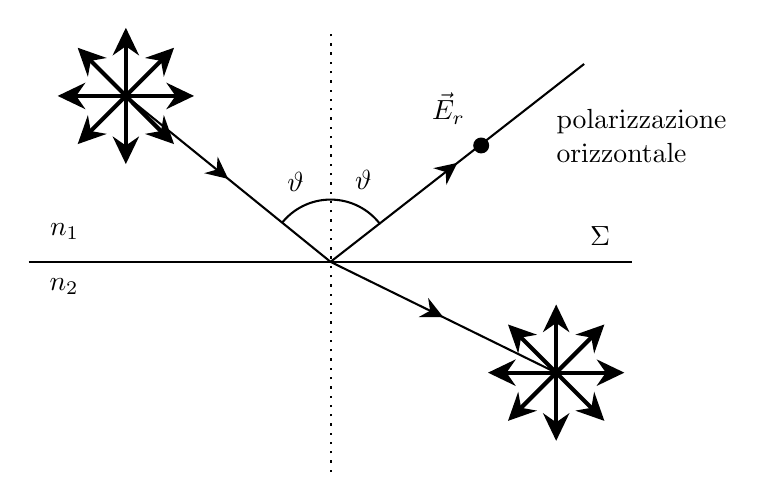
\begin{tikzpicture}[x=0.75pt,y=0.75pt,yscale=-1,xscale=1]
	%uncomment if require: \path (0,300); %set diagram left start at 0, and has height of 300

	%Straight Lines [id:da10584314933739614] 
	\draw [line width=0.75]    (186.08,178) -- (476.92,178) ;
	%Straight Lines [id:da6776483318154041] 
	\draw [line width=1.5]    (212.5,77.67) -- (253.27,118.45) ;
	\draw [shift={(256.09,121.27)}, rotate = 225] [fill={rgb, 255:red, 0; green, 0; blue, 0 }  ][line width=0.08]  [draw opacity=0] (13.4,-6.43) -- (0,0) -- (13.4,6.44) -- (8.9,0) -- cycle    ;
	\draw [shift={(209.67,74.85)}, rotate = 45] [fill={rgb, 255:red, 0; green, 0; blue, 0 }  ][line width=0.08]  [draw opacity=0] (13.4,-6.43) -- (0,0) -- (13.4,6.44) -- (8.9,0) -- cycle    ;
	%Shape: Circle [id:dp5620783808094743] 
	\draw  [fill={rgb, 255:red, 0; green, 0; blue, 0 }  ,fill opacity=1 ] (400.75,121.93) .. controls (400.75,120.09) and (402.24,118.6) .. (404.08,118.6) .. controls (405.92,118.6) and (407.42,120.09) .. (407.42,121.93) .. controls (407.42,123.77) and (405.92,125.26) .. (404.08,125.26) .. controls (402.24,125.26) and (400.75,123.77) .. (400.75,121.93) -- cycle ;
	%Straight Lines [id:da5967449817586901] 
	\draw [line width=0.75]  [dash pattern={on 0.84pt off 2.51pt}]  (331.5,279.25) -- (331.5,67) ;
	%Straight Lines [id:da2020356289457561] 
	\draw [line width=1.5]    (232.88,69.23) -- (232.88,126.89) ;
	\draw [shift={(232.88,130.89)}, rotate = 270] [fill={rgb, 255:red, 0; green, 0; blue, 0 }  ][line width=0.08]  [draw opacity=0] (13.4,-6.43) -- (0,0) -- (13.4,6.44) -- (8.9,0) -- cycle    ;
	\draw [shift={(232.88,65.23)}, rotate = 90] [fill={rgb, 255:red, 0; green, 0; blue, 0 }  ][line width=0.08]  [draw opacity=0] (13.4,-6.43) -- (0,0) -- (13.4,6.44) -- (8.9,0) -- cycle    ;
	%Straight Lines [id:da3215170377627532] 
	\draw [line width=1.5]    (253.27,77.67) -- (212.5,118.45) ;
	\draw [shift={(209.67,121.27)}, rotate = 315] [fill={rgb, 255:red, 0; green, 0; blue, 0 }  ][line width=0.08]  [draw opacity=0] (13.4,-6.43) -- (0,0) -- (13.4,6.44) -- (8.9,0) -- cycle    ;
	\draw [shift={(256.09,74.85)}, rotate = 135] [fill={rgb, 255:red, 0; green, 0; blue, 0 }  ][line width=0.08]  [draw opacity=0] (13.4,-6.43) -- (0,0) -- (13.4,6.44) -- (8.9,0) -- cycle    ;
	%Straight Lines [id:da6609842584002097] 
	\draw [line width=1.5]    (261.71,98.06) -- (204.05,98.06) ;
	\draw [shift={(200.05,98.06)}, rotate = 360] [fill={rgb, 255:red, 0; green, 0; blue, 0 }  ][line width=0.08]  [draw opacity=0] (13.4,-6.43) -- (0,0) -- (13.4,6.44) -- (8.9,0) -- cycle    ;
	\draw [shift={(265.71,98.06)}, rotate = 180] [fill={rgb, 255:red, 0; green, 0; blue, 0 }  ][line width=0.08]  [draw opacity=0] (13.4,-6.43) -- (0,0) -- (13.4,6.44) -- (8.9,0) -- cycle    ;
	%Straight Lines [id:da020335654979837248] 
	\draw [line width=0.75]    (232.88,98.06) -- (331.5,178) ;
	\draw [shift={(282.19,138.03)}, rotate = 219.03] [fill={rgb, 255:red, 0; green, 0; blue, 0 }  ][line width=0.08]  [draw opacity=0] (10.72,-5.15) -- (0,0) -- (10.72,5.15) -- (7.12,0) -- cycle    ;
	%Straight Lines [id:da601886995433131] 
	\draw [line width=1.5]    (419.83,211.01) -- (460.6,251.78) ;
	\draw [shift={(463.43,254.61)}, rotate = 225] [fill={rgb, 255:red, 0; green, 0; blue, 0 }  ][line width=0.08]  [draw opacity=0] (13.4,-6.43) -- (0,0) -- (13.4,6.44) -- (8.9,0) -- cycle    ;
	\draw [shift={(417,208.18)}, rotate = 45] [fill={rgb, 255:red, 0; green, 0; blue, 0 }  ][line width=0.08]  [draw opacity=0] (13.4,-6.43) -- (0,0) -- (13.4,6.44) -- (8.9,0) -- cycle    ;
	%Straight Lines [id:da3974384306150227] 
	\draw [line width=1.5]    (440.21,202.56) -- (440.21,260.22) ;
	\draw [shift={(440.21,264.22)}, rotate = 270] [fill={rgb, 255:red, 0; green, 0; blue, 0 }  ][line width=0.08]  [draw opacity=0] (13.4,-6.43) -- (0,0) -- (13.4,6.44) -- (8.9,0) -- cycle    ;
	\draw [shift={(440.21,198.56)}, rotate = 90] [fill={rgb, 255:red, 0; green, 0; blue, 0 }  ][line width=0.08]  [draw opacity=0] (13.4,-6.43) -- (0,0) -- (13.4,6.44) -- (8.9,0) -- cycle    ;
	%Straight Lines [id:da2923488269969061] 
	\draw [line width=1.5]    (460.6,211.01) -- (419.83,251.78) ;
	\draw [shift={(417,254.61)}, rotate = 315] [fill={rgb, 255:red, 0; green, 0; blue, 0 }  ][line width=0.08]  [draw opacity=0] (13.4,-6.43) -- (0,0) -- (13.4,6.44) -- (8.9,0) -- cycle    ;
	\draw [shift={(463.43,208.18)}, rotate = 135] [fill={rgb, 255:red, 0; green, 0; blue, 0 }  ][line width=0.08]  [draw opacity=0] (13.4,-6.43) -- (0,0) -- (13.4,6.44) -- (8.9,0) -- cycle    ;
	%Straight Lines [id:da0769012257333288] 
	\draw [line width=1.5]    (469.04,231.39) -- (411.38,231.39) ;
	\draw [shift={(407.38,231.39)}, rotate = 360] [fill={rgb, 255:red, 0; green, 0; blue, 0 }  ][line width=0.08]  [draw opacity=0] (13.4,-6.43) -- (0,0) -- (13.4,6.44) -- (8.9,0) -- cycle    ;
	\draw [shift={(473.04,231.39)}, rotate = 180] [fill={rgb, 255:red, 0; green, 0; blue, 0 }  ][line width=0.08]  [draw opacity=0] (13.4,-6.43) -- (0,0) -- (13.4,6.44) -- (8.9,0) -- cycle    ;
	%Straight Lines [id:da16469269400468023] 
	\draw [line width=0.75]    (331.5,178) -- (440.21,231.39) ;
	\draw [shift={(385.86,204.7)}, rotate = 206.16] [fill={rgb, 255:red, 0; green, 0; blue, 0 }  ][line width=0.08]  [draw opacity=0] (10.72,-5.15) -- (0,0) -- (10.72,5.15) -- (7.12,0) -- cycle    ;
	%Straight Lines [id:da0759372633547084] 
	\draw [line width=0.75]    (331.5,178) -- (453.67,82.67) ;
	\draw [shift={(392.58,130.33)}, rotate = 502.03] [fill={rgb, 255:red, 0; green, 0; blue, 0 }  ][line width=0.08]  [draw opacity=0] (10.72,-5.15) -- (0,0) -- (10.72,5.15) -- (7.12,0) -- cycle    ;
	%Shape: Arc [id:dp652910950328399] 
	\draw  [draw opacity=0] (308,159.35) .. controls (313.5,152.43) and (321.98,148) .. (331.5,148) .. controls (341.27,148) and (349.96,152.68) .. (355.44,159.91) -- (331.5,178) -- cycle ; \draw   (308,159.35) .. controls (313.5,152.43) and (321.98,148) .. (331.5,148) .. controls (341.27,148) and (349.96,152.68) .. (355.44,159.91) ;

	% Text Node
	\draw (203.33,163.33) node    {$n_{1}$};
	% Text Node
	\draw (205.33,190) node    {$n_{2} \ $};
	% Text Node
	\draw (461.33,165.33) node    {$\Sigma $};
	% Text Node
	\draw (388.33,104.17) node    {$\vec{E}_{r}$};
	% Text Node
	\draw (314.67,139.33) node    {$\vartheta $};
	% Text Node
	\draw (347.33,138.67) node    {$\vartheta $};
	% Text Node
	\draw (481.33,117.33) node   [align=left] {polarizzazione\\orizzontale};

	\end{tikzpicture}
\end{figure}
\FloatBarrier

\section{Incidenza normale alla superficie di separazione}

Quando l'angolo di incidenza è nullo la direzione di incidenza coincide con la normale alla superficie di separazione e la nozione di piano di incidenza perde significato. I campi elettrici dell'onda incidente, dell'onda riflessa e dell'onda trasmessa sono paralleli tra loro e alla superficie e le condizioni al contorno si riducono all'unica condizione:

\[
	\vec{E}_i+\vec{E}_r = \vec{E}_t
\]

Le formule di Fresnel saranno:

\[
	\boxed{r = \frac{E_r}{E_i} = \frac{n_1-n_2}{n_1+n_2} \qquad t = \frac{E_t}{E_i}= \frac{2n_1}{n_1+n_2}}
\]

Mentre $t$ è sempre positivo, $r$ è negativo se $n_1<n_2$ e positivo in caso contrario. Nel primo caso (es aria-vetro) il campo elettrico riflesso è opposto al campo elettrico incidente (sfasamento di $\pi$). Nel secondo caso campo elettrico riflesso e incidente sono concordi (in fase).

\begin{figure}[htpb]
	\centering

	\tikzset{every picture/.style={line width=0.75pt}} %set default line width to 0.75pt        

	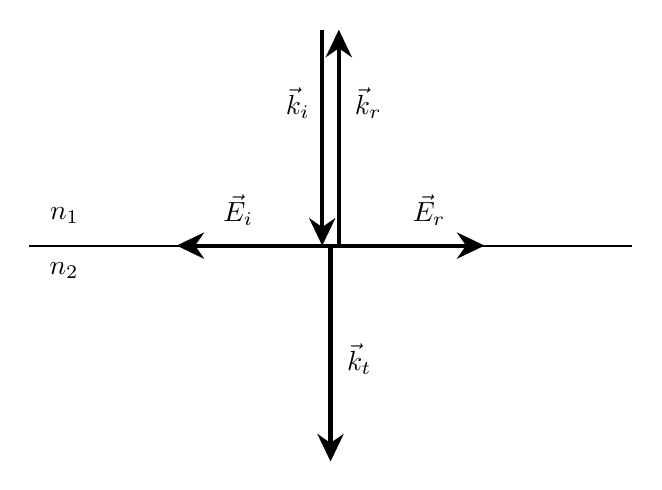
\begin{tikzpicture}[x=0.75pt,y=0.75pt,yscale=-1,xscale=1]
	%uncomment if require: \path (0,300); %set diagram left start at 0, and has height of 300

	%Straight Lines [id:da8343733937814433] 
	\draw [line width=0.75]    (185.42,166.67) -- (476.25,166.67) ;
	%Straight Lines [id:da9542436852727807] 
	\draw [line width=1.5]    (326.83,62.67) -- (326.83,162.67) ;
	\draw [shift={(326.83,166.67)}, rotate = 270] [fill={rgb, 255:red, 0; green, 0; blue, 0 }  ][line width=0.08]  [draw opacity=0] (13.4,-6.43) -- (0,0) -- (13.4,6.44) -- (8.9,0) -- cycle    ;
	%Straight Lines [id:da124426243237312] 
	\draw [line width=1.5]    (334.83,66.67) -- (334.83,166.67) ;
	\draw [shift={(334.83,62.67)}, rotate = 90] [fill={rgb, 255:red, 0; green, 0; blue, 0 }  ][line width=0.08]  [draw opacity=0] (13.4,-6.43) -- (0,0) -- (13.4,6.44) -- (8.9,0) -- cycle    ;
	%Straight Lines [id:da1865350143004918] 
	\draw [line width=1.5]    (330.83,166.67) -- (330.83,266.67) ;
	\draw [shift={(330.83,270.67)}, rotate = 270] [fill={rgb, 255:red, 0; green, 0; blue, 0 }  ][line width=0.08]  [draw opacity=0] (13.4,-6.43) -- (0,0) -- (13.4,6.44) -- (8.9,0) -- cycle    ;
	%Straight Lines [id:da2872402626087014] 
	\draw [line width=1.5]    (330.83,166.67) -- (401,166.67) ;
	\draw [shift={(405,166.67)}, rotate = 180] [fill={rgb, 255:red, 0; green, 0; blue, 0 }  ][line width=0.08]  [draw opacity=0] (13.4,-6.43) -- (0,0) -- (13.4,6.44) -- (8.9,0) -- cycle    ;
	%Straight Lines [id:da8246612781024789] 
	\draw [line width=1.5]    (260.67,166.67) -- (330.83,166.67) ;
	\draw [shift={(256.67,166.67)}, rotate = 0] [fill={rgb, 255:red, 0; green, 0; blue, 0 }  ][line width=0.08]  [draw opacity=0] (13.4,-6.43) -- (0,0) -- (13.4,6.44) -- (8.9,0) -- cycle    ;

	% Text Node
	\draw (202.67,152) node    {$n_{1}$};
	% Text Node
	\draw (204.67,178.67) node    {$n_{2} \ $};
	% Text Node
	\draw (344.67,221.33) node    {$\vec{k}_{t}$};
	% Text Node
	\draw (349,98) node    {$\vec{k}_{r}$};
	% Text Node
	\draw (315,98) node    {$\vec{k}_{i}$};
	% Text Node
	\draw (378.33,149.67) node    {$\vec{E}_{r}$};
	% Text Node
	\draw (286.33,149.67) node    {$\vec{E}_{i}$};

	\end{tikzpicture}
\end{figure}
\FloatBarrier

\section{Riflessione su una superficie metallica}

Le equazioni di Fresnel si possono usare anche quando il materiale assorbe (quindi quando l'indice di rifrazione è complesso). Il caso più interessante è quello in cui tale materiale è un conduttore. Ivi non c'è la forza di richiamo che avevamo introdotto nel caso della propagazione delle onde elettromagnetiche nel dielettrico: gli elettroni di conduzione infatti sono liberi. Possiamo quindi usare la formula dell'indice di rifrazione complesso ponendo $\omega_0=0$. Se non ci sono effetti dissipativi (conducibilità infinita) anche il coefficiente di attrito viscoso può essere posto pari a $0$. A questo punto l'indice di rifrazione di un metallo perfetto si può scrivere nella forma:

\begin{align*}
	n(\omega) &= \sqrt{1+\frac{Ne^2 (\omega_0^2 -\omega^2)-i\gamma \omega}{m_e\varepsilon_0 (\omega_0^2 -\omega^2)^2 + \gamma^2 \omega^2}} \tag*{$\gamma=0,\omega_0=0$}\\
	&= \sqrt{1+\frac{Ne^2}{m_e\varepsilon_0}\frac{(-\omega^2)}{\omega^4}}\\
	&= \sqrt{1-\frac{Ne^2}{m_e\varepsilon_0 \omega^2}}
\end{align*}

In questa situazione si introduce una quantità detta \textbf{pulsazione di plasma} del metallo. Essa è data dal rapporto:

\[
	\omega_p = \sqrt{\frac{Ne^2}{m_e\varepsilon_0}} \qquad \text{pulsazione di plasma}
\]

L'indice di rifrazione complesso si scrive allora come:

\[
	n(\omega) = \sqrt{1-\frac{\omega_p^2}{\omega^2}}
\]

Studiamo il segno della quantità sotto radice.

\begin{itemize}
	\item Per $\omega<\omega_p\implies n=i\,n_I(\omega)$. In tal caso la quantità sotto radice è negativa e l'indice di rifrazione è solo immaginario, il che comporta che non ci può essere propagazione nel metallo, ma solo assorbimento di energia.
	\item Per $\omega>\omega_p\implies n=i\,n_R(\omega)$. In tal caso la quantità sotto radice è positiva e l'indice di rifrazione è solo reale, non c'è assorbimento e il metallo diventa trasparente alle onde.
\end{itemize}

Dal momento che le pulsazioni di plasma hanno valori dell'ordine di $10^{16}\,rad/s$, le pulsazioni visibili obbediscono alla $\omega<\omega_p$ e quindi l'indice di rifrazione ha un valore immaginario puro. Sappiamo già che in questa situazione non può esserci propagazione nel metallo. Si possono usare le equazioni di Fresnel per dimostrare che una superficie metallica riflette quasi tutta l'energia luminosa che la colpisce:

\[
	\frac{E_r}{E_i} = \frac{n_1-n_2}{n_1+n_2} = \frac{1-in_I}{1+in_I} = \frac{\rho e^{-i\varphi}}{\rho e^{i\varphi}} = e^{-2i\varphi} \implies \left|\frac{E_r}{E_i}\right|^2 = \frac{I_r}{I_i} = \left( e^{-2i\varphi}  \right)^2 = 1
\]

I metalli che hanno il maggior coefficiente di riflessione nel visibile, sono l'argento e l'alluminio. Il fenomeno di riflessione delle onde elettromagnetiche su una superficie metallica è alla base del funzionamento degli specchi. Dato che l'alluminio, se esposto all'aria per tempi molto lunghi, resta sostanzialmente inalterato a differenza dell'argento, gli specchi vengono fatti preferibilmente con una sottile pellicola di alluminio.

\section{Cenni ai fenomeni di interferenza fra onde elettromagnetiche}

Tutti i fenomeni di tipo ondulatorio generalmente sono associati a fenomeni di interferenza, termine riferito alla sovrapposizione di due o più onde elettromagnetiche della stessa natura. Per parlare di tale argomento, dobbiamo introdurre il concetto di \textbf{coerenza} fra due onde elettromagnetiche. Immaginiamo due di queste sinusoidali e piane che nella stessa regione di spazio si sovrappongono.

\[
	\vec{E}_1(\vec{r},t) = \vec{E}_{01}\cos (\underbrace{\vec{k}_1\cdot \vec{r} -\omega_1 t + \varphi_1}_{\Phi_1}) \qquad \vec{E}_2(\vec{r},t) = \vec{E}_{02}\cos (\underbrace{\vec{k}_2\cdot \vec{r} -\omega_2 t + \varphi_2}_{\Phi_2})
\]

Diremo che due onde elettromagnetiche sono fra loro coerenti se la differenza tra le due fasi non dipende dal tempo.

\[
	\Delta \Phi = \Phi_1 (\vec{r},t) - \Phi_2 (\vec{r}, t)
\]

Per analogia, sorgenti che generano onde coerenti sono a loro volta dette coerenti.
Se vogliamo che le onde siano coerenti, dobbiamo fare in modo che $t$ non compaia nell'espressione di $ \Delta \Phi  $

\[
	\Delta \Phi = (\vec{k}_1 - \vec{k}_2)\vec{r} -(\omega_1 - \omega_2) t + (\varphi_1 - \varphi _2  )
\]

Dobbiamo quindi prima di tutto richiedere che le due frequenze siano le stesse. Inoltre, quando si estende la trattazione a onde non polarizzate, $\varphi_1$ e $\varphi_2$ potrebbero variare nel tempo. Quindi si richiede anche che la loro differenza sia costante.\\
\textbf{Osservazione.} Si utilizzano sorgenti laser per ottenere onde coerenti.
Poniamo che ci siano due onde piane sinusoidali coerenti linearmente polarizzate nella stessa direzione (ad esempio l'asse $y$).

\[
	\vec{E}_1(\vec{r},t) = E_{01} \vec{u}_y \cos (\Phi_1) \qquad \vec{E}_2(\vec{r},t) = E_{02} \vec{u}_y \cos (\Phi_2)
\]

Avremo un'onda complessiva data dalla somma delle due onde. La loro sovrapposizione sarà:

\[
	\vec{E} (\vec{r},t) = \vec{E}_1(\vec{r},t) + \vec{E}_2(\vec{r},t)
\]

Chiediamoci quanto vale l'intensità di questa onda complessiva. L'intensità istantanea è pari al modulo del vettore di Poynting.

\begin{equation*}
	\begin{aligned}
		I(\vec{r},t) = |\vec{S}| &= \varepsilon_0 \varepsilon_r v |\vec{E}|^2 \\
		&=\varepsilon_0 \varepsilon_r v \left\{ E_{01}\cos (\Phi_1) + E_{02}\cos (\Phi_2 )  \right\}^2 \\
		&= \varepsilon_0 \varepsilon_r v \left\{ E_{01}^2 \cos^2 (\Phi_1 ) + E_{02}^2 \cos^2 (\Phi_2 ) + 2 E_{01}E_{02}\cos (\Phi_1 )\cos (\Phi_2 ) \right\} \\
		&= \varepsilon_0 \varepsilon_r v \{ E_{01}^2 \cos^2 (\Phi_1 ) + E_{02}^2 \cos^2 (\Phi_2 ) + E_{01}E_{02}\cos (\Phi_1 + \Phi_2) \\
		&\qquad\qquad + E_{01}E_{02}\cos (\Phi_1 - \Phi_2) \}
	\end{aligned}
\end{equation*}

Il valor medio del terzo termine è nullo perché si tratta di una funzione oscillante intorno allo zero. Il quarto non è in realtà una funzione oscillante perché, essendo le due onde coerenti, la differenza fra le fasi non dipende dal tempo ma è una costante.
Tenendo conto che il valor medio del coseno al quadrato è pari a 1/2, l'intensità media sarà data da:

\[
	I_m = \varepsilon_0 \varepsilon_r v \left\{ \frac{E_{01}^2}{2} + \frac{E_{02}^2}{2} + E_{01}E_{02} \cos (\Delta \Phi) \right\}
\]

Osserviamo che l'intensità rispettivamente delle due onde è data da:

\[
	I_{m1} = \frac{1}{2} \varepsilon_0 \varepsilon_r v E_{01}^2 \qquad I_{m2} = \frac{1}{2} \varepsilon_0 \varepsilon_r v E_{02}^2
\]

Si può dimostrare che

\[
	\varepsilon_0 \varepsilon_r v E_{02}E_{02} = 2 \sqrt{I_{m1}I_{m2}}
\]

L'intensità media totale sarà quindi

\[
	I_m = I_{m1} + I_{m2} + 2 \sqrt{I_{m1}I_{m2}} \cos (\Delta \Phi)
\]

Quando l'intensità totale dipende dalla differenza di fase fra le due onde elettromagnetiche, si parla di fenomeno di interferenza. L'intensità complessiva dovuta alla sovrapposizione delle due onde dipende dalla differenza di fase e non si ottiene come semplice somma delle singole intensità medie.
Quando le due onde non sono coerenti, anche la differenza di fase sarà funzione del tempo. Calcolando il valor medio della parte sottolineata in blu, esso verrebbe zero perché la funzione oscillerebbe. Per onde incoerenti, l'intensità totale è la somma delle intensità delle due onde. Si parla di sorgenti incoerenti quando esse generando onde incoerenti.
Affinché si manifestino fenomeni di interferenza, è molto importante che la direzione di polarizzazione sia la stessa. Consideriamo ad esempio due onde coerenti con polarizzazione ortogonale. Il campo elettrico sarà dato da:

\[
	\vec{E} (\vec{r},t) = E_{01}\vec{u}_y\cos (\vec{k}_1\cdot \vec{r} -\omega t + \varphi_1  ) + E_{02}\vec{u}_z\cos (\vec{k}_2\cdot \vec{r} -\omega t + \varphi_2  )
\]

Quando calcoliamo l'intensità istantanea abbiamo:

\[
	I = \varepsilon_0 \varepsilon_r v |\vec{E}|^2 = \varepsilon_0 \varepsilon_r v(\vec{E} \cdot \vec{E})
\]

Calcolando il prodotto scalare avremmo in teoria quattro termini. Quelli in cui compare il prodotto scalare fra i due versori $ \vec{u}_z $ e $ \vec{u}_y $ sono pari a zero. Risulterà:

\[
	I = E_{01}^2 \cos^2 (\vec{k}_1\cdot \vec{r} -\omega t + \varphi_1) + E_{02}^2 \cos^2 (\vec{k}_2+\omega t + \varphi_2 = I_{m1}+I_{m2}
\]

Le onde devono quindi essere polarizzate lungo la stessa direzione perché possa comparire il doppio prodotto fra la loro intensità.
Consideriamo il semplice caso in cui le due onde hanno la stessa intensità $ I_{m1}=I_{m2}=I_0    $.

\[
	I=I_0+I_0+2\sqrt{I_0^2} \cos \left[ \Delta \Phi (\vec{r}) \right] = 2I_0 \left[ 1+\cos \Delta \Phi (\vec{r}) \right]
\]

Vediamo che cosa può accadere a questa quantità in due casi diversi.

\begin{itemize}
	\item \textbf{Caso 1.} La fase è un multiplo pari di $ \pi  $.
	\[
		\Delta \Phi = 2\pi m\qquad m=0,\pm 1,\pm 2\ldots  \implies \cos [\Delta \Phi ]=1 \quad I=4I_0
	\]
	Si parla in tal caso di \textbf{interferenza costruttiva}: le onde sono in fase: la differenza di cammino è un multiplo intero della lunghezza d'onda.
	\begin{figure}[htpb]
		\centering
		

		\tikzset{every picture/.style={line width=0.75pt}} %set default line width to 0.75pt        

		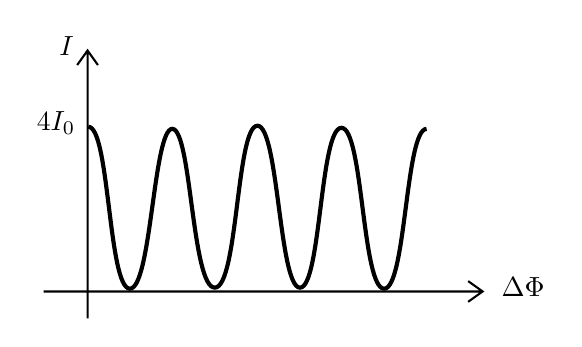
\begin{tikzpicture}[x=0.75pt,y=0.75pt,yscale=-1,xscale=1]
		%uncomment if require: \path (0,300); %set diagram left start at 0, and has height of 300

		%Curve Lines [id:da925891687150687] 
		\draw [line width=1.5]    (214.5,101.75) .. controls (224.71,101.5) and (224.14,179.5) .. (234.5,179.75) .. controls (244.86,180) and (245.86,102.64) .. (255,102.75) .. controls (264.14,102.86) and (264.43,179.5) .. (275.5,179.25) .. controls (286.57,179) and (285.86,101.21) .. (296,101.25) .. controls (306.14,101.29) and (306.43,179.21) .. (316.5,179.25) .. controls (326.57,179.29) and (326.14,102.07) .. (336.5,102.25) .. controls (346.86,102.43) and (346.43,179.5) .. (357,179.75) .. controls (367.57,180) and (367.29,102.64) .. (377.5,102.75) ;
		%Shape: Axis 2D [id:dp85463191663918] 
		\draw  (193,181.1) -- (404.5,181.1)(214.15,65) -- (214.15,194) (397.5,176.1) -- (404.5,181.1) -- (397.5,186.1) (209.15,72) -- (214.15,65) -- (219.15,72)  ;

		% Text Node
		\draw (424,179) node    {$\Delta \Phi $};
		% Text Node
		\draw (204,63) node    {$I$};
		% Text Node
		\draw (199,100) node    {$4I_{0}$};

		\end{tikzpicture}
	\end{figure}
	\FloatBarrier

	\item \textbf{Caso 2.} La fase è un multiplo dispari di $ \pi  $.
	\[
		\Delta \Phi = (2m+1)\pi \implies \cos [\Delta \Phi ]=-1 \quad I=0
	\]
	In tal caso si parla di \textbf{interferenza distruttiva}. Le onde sono in opposizione di fase e ciò comporta che la differenza di cammino sia un multiplo dispari di mezza lunghezza d'onda. In tutti gli altri casi In l'intensità totale varia fra questi due estremi.
\end{itemize}

\section{Interferenza fra onde emesse da due sorgenti luminose puntiformi}

Un tipico esempio di sorgente puntiforme di onde elettromagnetiche è una stella. Immaginiamo che la potenza irradiata dalla sorgente sia $W_0$.

\begin{figure}[htpb]
	\centering

	\tikzset{every picture/.style={line width=0.75pt}} %set default line width to 0.75pt        

	\begin{tikzpicture}[x=0.75pt,y=0.75pt,yscale=-0.8,xscale=0.8]
	%uncomment if require: \path (0,300); %set diagram left start at 0, and has height of 300

	%Shape: Circle [id:dp7799479554093001] 
	\draw  [dash pattern={on 0.84pt off 2.51pt}] (243,165.75) .. controls (243,135.51) and (267.51,111) .. (297.75,111) .. controls (327.99,111) and (352.5,135.51) .. (352.5,165.75) .. controls (352.5,195.99) and (327.99,220.5) .. (297.75,220.5) .. controls (267.51,220.5) and (243,195.99) .. (243,165.75) -- cycle ;
	%Straight Lines [id:da746600712772753] 
	\draw  [dash pattern={on 0.84pt off 2.51pt}]  (297.75,165.75) -- (259.04,127.04) ;

	% Text Node
	\draw (291,139) node    {$r$};
	% Text Node
	\draw (215,127) node    {$P$};
	% Text Node
	\draw (314,202) node    {$S$};

	\end{tikzpicture}
\end{figure}
\FloatBarrier

Poniamo di voler calcolare l'intensità della radiazione che giunge nel punto $P$. La sorgente puntiforme irradia potenza in tutte le direzioni in modo uniforme, è sufficiente pensare che essa si distribuisce in una superficie sferica di raggio $r$, quindi l'intensità si può calcolare semplicemente come:

\[
	I=\frac{W_0}{4\pi r^2}
\]

Essa decresce con il quadrato della distanza perché si distribuisce su una superficie sempre più grande. Siccome $I$ è uguale in modulo al vettore di Poynting, che è proporzionale al modulo del campo elettrico dell'onda al quadrato, $\vec{E}$ deve decrescere come $1/r$. L'onda elettromagnetica emessa prende il nome di \textbf{onda sferica}. Le sue caratteristiche sono:

\begin{itemize}
	\item $\vec{E}$ decresce con la distanza.
	\item Mentre nelle onde piane ha senso parlare di direzione di propagazione, nel caso di un'onda sferica non c'è direzione specifica per identificarla. In questo caso useremo il modulo del vettore $\vec{k} $.
\end{itemize}

Le onde sferiche si possono identificare in questo modo:

\[
	E(\vec{r},t) = \frac{A}{r} \cos (kr-\omega t)
\]

A questo punto se abbiamo due sorgenti puntiformi e vogliamo studiare il fenomeno di interferenza nel punto $P$ procediamo calcolando le intensità delle radiazioni nel punto $P$ emesse da $S_1$ ed $S_2$ rispettivamente.

\begin{gather*}
	I_1(P) = \frac{W_0}{4\pi r_1^2} \qquad I_2(P) = \frac{W_0}{4\pi r_2^2} \\
	I(P) = I_1(P) + I_2(P) + 2\sqrt{I_1I_2} \cos \Delta \Phi \\
	\Delta \Phi = kr_1-kr_2 = k(r_1-r_2  )
\end{gather*}

Vediamo quando si ha interferenza costruttiva:

\begin{align*}
	\Delta \Phi &= 2\pi m \\
	k(r_1-r_2) &= 2\pi m \\
	\frac{2\pi}{\lambda}(r_1-r_2) &= 2\pi m \\
	\frac{1}{\lambda}(r_1-r_2) &= m \\
	\Aboxed{r_1-r_2 &= m\lambda}
\end{align*}

Si trova l'equazione di una famiglia di iperboli. A seconda del valore di m avremo differenti iperboli, i cui fuochi si trovano sempre su $S_1$ ed $S_2$. Tali curve sono il luogo dei punti in cui si ha interferenza costruttiva.

\begin{figure}[htpb]
	\centering

	\tikzset{every picture/.style={line width=0.75pt}} %set default line width to 0.75pt        

	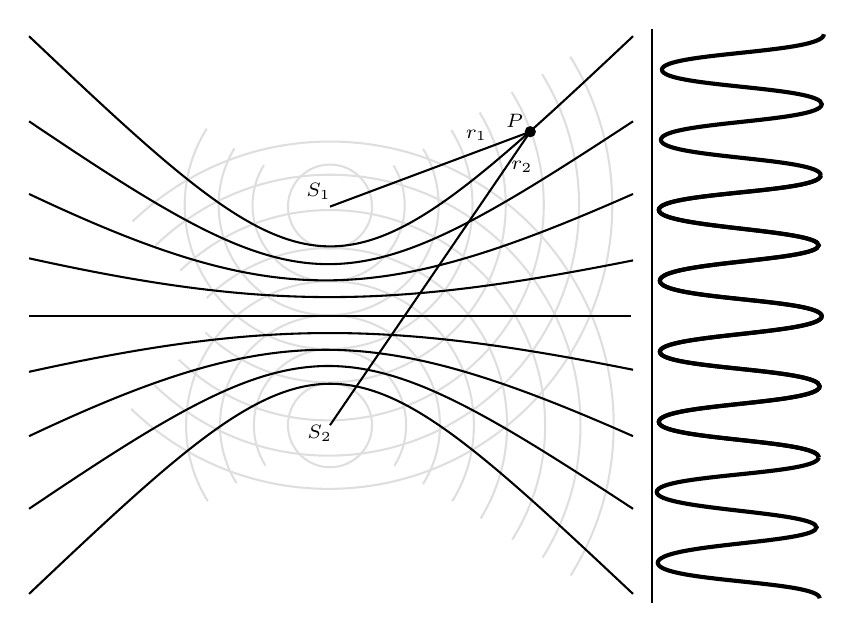
\begin{tikzpicture}[x=0.75pt,y=0.75pt,yscale=-1,xscale=1]
	%uncomment if require: \path (0,300); %set diagram left start at 0, and has height of 300

	%Shape: Circle [id:dp08060543997148284] 
	\draw  [color={rgb, 255:red, 222; green, 222; blue, 222 }  ,draw opacity=1 ] (265,74.09) .. controls (276.19,74.09) and (285.25,83.16) .. (285.25,94.34) .. controls (285.25,105.53) and (276.19,114.6) .. (265,114.6) .. controls (253.81,114.6) and (244.75,105.53) .. (244.75,94.34) .. controls (244.75,83.16) and (253.81,74.09) .. (265,74.09) -- cycle ;
	%Shape: Circle [id:dp3870702516407525] 
	\draw  [color={rgb, 255:red, 222; green, 222; blue, 222 }  ,draw opacity=1 ] (265,179.4) .. controls (276.19,179.4) and (285.25,188.47) .. (285.25,199.66) .. controls (285.25,210.84) and (276.19,219.91) .. (265,219.91) .. controls (253.81,219.91) and (244.75,210.84) .. (244.75,199.66) .. controls (244.75,188.47) and (253.81,179.4) .. (265,179.4) -- cycle ;
	%Shape: Arc [id:dp7818118033781998] 
	\draw  [draw opacity=0] (233.92,219.13) .. controls (230.38,213.49) and (228.33,206.81) .. (228.33,199.66) .. controls (228.33,179.41) and (244.75,162.99) .. (265,162.99) .. controls (285.25,162.99) and (301.67,179.41) .. (301.67,199.66) .. controls (301.67,206.83) and (299.61,213.52) .. (296.04,219.18) -- (265,199.66) -- cycle ; \draw  [color={rgb, 255:red, 222; green, 222; blue, 222 }  ,draw opacity=1 ] (233.92,219.13) .. controls (230.38,213.49) and (228.33,206.81) .. (228.33,199.66) .. controls (228.33,179.41) and (244.75,162.99) .. (265,162.99) .. controls (285.25,162.99) and (301.67,179.41) .. (301.67,199.66) .. controls (301.67,206.83) and (299.61,213.52) .. (296.04,219.18) ;
	%Shape: Arc [id:dp2550254959984686] 
	\draw  [draw opacity=0] (219.96,227.58) .. controls (214.92,219.47) and (212.01,209.91) .. (212.01,199.66) .. controls (212.01,170.39) and (235.73,146.67) .. (265,146.67) .. controls (294.27,146.67) and (317.99,170.39) .. (317.99,199.66) .. controls (317.99,210.08) and (314.98,219.8) .. (309.79,227.99) -- (265,199.66) -- cycle ; \draw  [color={rgb, 255:red, 222; green, 222; blue, 222 }  ,draw opacity=1 ] (219.96,227.58) .. controls (214.92,219.47) and (212.01,209.91) .. (212.01,199.66) .. controls (212.01,170.39) and (235.73,146.67) .. (265,146.67) .. controls (294.27,146.67) and (317.99,170.39) .. (317.99,199.66) .. controls (317.99,210.08) and (314.98,219.8) .. (309.79,227.99) ;
	%Shape: Arc [id:dp06300146565821207] 
	\draw  [draw opacity=0] (206.14,236.32) .. controls (199.5,225.68) and (195.67,213.12) .. (195.67,199.66) .. controls (195.67,161.36) and (226.71,130.32) .. (265,130.32) .. controls (303.29,130.32) and (334.33,161.36) .. (334.33,199.66) .. controls (334.33,213.1) and (330.51,225.65) .. (323.88,236.28) -- (265,199.66) -- cycle ; \draw  [color={rgb, 255:red, 222; green, 222; blue, 222 }  ,draw opacity=1 ] (206.14,236.32) .. controls (199.5,225.68) and (195.67,213.12) .. (195.67,199.66) .. controls (195.67,161.36) and (226.71,130.32) .. (265,130.32) .. controls (303.29,130.32) and (334.33,161.36) .. (334.33,199.66) .. controls (334.33,213.1) and (330.51,225.65) .. (323.88,236.28) ;
	%Shape: Arc [id:dp9877380941575995] 
	\draw  [draw opacity=0] (205.6,138.39) .. controls (220.97,123.49) and (241.91,114.32) .. (265,114.32) .. controls (312.13,114.32) and (350.33,152.53) .. (350.33,199.66) .. controls (350.33,216.16) and (345.65,231.56) .. (337.54,244.62) -- (265,199.66) -- cycle ; \draw  [color={rgb, 255:red, 222; green, 222; blue, 222 }  ,draw opacity=1 ] (205.6,138.39) .. controls (220.97,123.49) and (241.91,114.32) .. (265,114.32) .. controls (312.13,114.32) and (350.33,152.53) .. (350.33,199.66) .. controls (350.33,216.16) and (345.65,231.56) .. (337.54,244.62) ;
	%Shape: Arc [id:dp5004358798621307] 
	\draw  [draw opacity=0] (192.85,125.23) .. controls (211.51,107.14) and (236.96,96) .. (265,96) .. controls (322.25,96) and (368.66,142.41) .. (368.66,199.66) .. controls (368.66,219.93) and (362.84,238.85) .. (352.77,254.82) -- (265,199.66) -- cycle ; \draw  [color={rgb, 255:red, 222; green, 222; blue, 222 }  ,draw opacity=1 ] (192.85,125.23) .. controls (211.51,107.14) and (236.96,96) .. (265,96) .. controls (322.25,96) and (368.66,142.41) .. (368.66,199.66) .. controls (368.66,219.93) and (362.84,238.85) .. (352.77,254.82) ;
	%Shape: Arc [id:dp2166898603176528] 
	\draw  [draw opacity=0] (181.01,113.02) .. controls (202.73,91.95) and (232.35,78.99) .. (265,78.99) .. controls (331.64,78.99) and (385.67,133.01) .. (385.67,199.66) .. controls (385.67,223.07) and (379,244.93) .. (367.46,263.43) -- (265,199.66) -- cycle ; \draw  [color={rgb, 255:red, 222; green, 222; blue, 222 }  ,draw opacity=1 ] (181.01,113.02) .. controls (202.73,91.95) and (232.35,78.99) .. (265,78.99) .. controls (331.64,78.99) and (385.67,133.01) .. (385.67,199.66) .. controls (385.67,223.07) and (379,244.93) .. (367.46,263.43) ;
	%Shape: Arc [id:dp4781416417159392] 
	\draw  [draw opacity=0] (169.87,101.53) .. controls (194.48,77.67) and (228.02,62.99) .. (265,62.99) .. controls (340.48,62.99) and (401.67,124.18) .. (401.67,199.66) .. controls (401.67,226.23) and (394.08,251.04) .. (380.95,272.03) -- (265,199.66) -- cycle ; \draw  [color={rgb, 255:red, 222; green, 222; blue, 222 }  ,draw opacity=1 ] (169.87,101.53) .. controls (194.48,77.67) and (228.02,62.99) .. (265,62.99) .. controls (340.48,62.99) and (401.67,124.18) .. (401.67,199.66) .. controls (401.67,226.23) and (394.08,251.04) .. (380.95,272.03) ;
	%Shape: Arc [id:dp25918293710577345] 
	\draw  [draw opacity=0] (233.16,74.35) .. controls (229.68,79.96) and (227.67,86.58) .. (227.67,93.67) .. controls (227.67,113.92) and (244.08,130.33) .. (264.33,130.33) .. controls (284.58,130.33) and (301,113.92) .. (301,93.67) .. controls (301,86.67) and (299.04,80.12) .. (295.63,74.56) -- (264.33,93.67) -- cycle ; \draw  [color={rgb, 255:red, 222; green, 222; blue, 222 }  ,draw opacity=1 ] (233.16,74.35) .. controls (229.68,79.96) and (227.67,86.58) .. (227.67,93.67) .. controls (227.67,113.92) and (244.08,130.33) .. (264.33,130.33) .. controls (284.58,130.33) and (301,113.92) .. (301,93.67) .. controls (301,86.67) and (299.04,80.12) .. (295.63,74.56) ;
	%Shape: Arc [id:dp37519196802558397] 
	\draw  [draw opacity=0] (218.97,66.26) .. controls (214.13,74.26) and (211.34,83.64) .. (211.34,93.67) .. controls (211.34,122.93) and (235.07,146.66) .. (264.33,146.66) .. controls (293.6,146.66) and (317.32,122.93) .. (317.32,93.67) .. controls (317.32,83.75) and (314.6,74.46) .. (309.85,66.52) -- (264.33,93.67) -- cycle ; \draw  [color={rgb, 255:red, 222; green, 222; blue, 222 }  ,draw opacity=1 ] (218.97,66.26) .. controls (214.13,74.26) and (211.34,83.64) .. (211.34,93.67) .. controls (211.34,122.93) and (235.07,146.66) .. (264.33,146.66) .. controls (293.6,146.66) and (317.32,122.93) .. (317.32,93.67) .. controls (317.32,83.75) and (314.6,74.46) .. (309.85,66.52) ;
	%Shape: Arc [id:dp45144955151664035] 
	\draw  [draw opacity=0] (205.62,56.78) .. controls (198.89,67.46) and (195,80.11) .. (195,93.67) .. controls (195,131.96) and (226.04,163) .. (264.33,163) .. controls (302.63,163) and (333.67,131.96) .. (333.67,93.67) .. controls (333.67,80.4) and (329.94,68.01) .. (323.48,57.48) -- (264.33,93.67) -- cycle ; \draw  [color={rgb, 255:red, 222; green, 222; blue, 222 }  ,draw opacity=1 ] (205.62,56.78) .. controls (198.89,67.46) and (195,80.11) .. (195,93.67) .. controls (195,131.96) and (226.04,163) .. (264.33,163) .. controls (302.63,163) and (333.67,131.96) .. (333.67,93.67) .. controls (333.67,80.4) and (329.94,68.01) .. (323.48,57.48) ;
	%Shape: Arc [id:dp8154313281969809] 
	\draw  [draw opacity=0] (204.94,154.94) .. controls (220.3,169.83) and (241.25,179) .. (264.33,179) .. controls (311.46,179) and (349.67,140.79) .. (349.67,93.67) .. controls (349.67,77.31) and (345.06,62.02) .. (337.08,49.04) -- (264.33,93.67) -- cycle ; \draw  [color={rgb, 255:red, 222; green, 222; blue, 222 }  ,draw opacity=1 ] (204.94,154.94) .. controls (220.3,169.83) and (241.25,179) .. (264.33,179) .. controls (311.46,179) and (349.67,140.79) .. (349.67,93.67) .. controls (349.67,77.31) and (345.06,62.02) .. (337.08,49.04) ;
	%Shape: Arc [id:dp9855388845867168] 
	\draw  [draw opacity=0] (192.18,168.09) .. controls (210.84,186.19) and (236.29,197.32) .. (264.33,197.32) .. controls (321.58,197.32) and (367.99,150.91) .. (367.99,93.67) .. controls (367.99,73.67) and (362.33,55) .. (352.52,39.16) -- (264.33,93.67) -- cycle ; \draw  [color={rgb, 255:red, 222; green, 222; blue, 222 }  ,draw opacity=1 ] (192.18,168.09) .. controls (210.84,186.19) and (236.29,197.32) .. (264.33,197.32) .. controls (321.58,197.32) and (367.99,150.91) .. (367.99,93.67) .. controls (367.99,73.67) and (362.33,55) .. (352.52,39.16) ;
	%Shape: Arc [id:dp942189796709634] 
	\draw  [draw opacity=0] (180.34,180.31) .. controls (202.07,201.37) and (231.69,214.33) .. (264.33,214.33) .. controls (330.98,214.33) and (385,160.31) .. (385,93.67) .. controls (385,70.53) and (378.49,48.92) .. (367.2,30.56) -- (264.33,93.67) -- cycle ; \draw  [color={rgb, 255:red, 222; green, 222; blue, 222 }  ,draw opacity=1 ] (180.34,180.31) .. controls (202.07,201.37) and (231.69,214.33) .. (264.33,214.33) .. controls (330.98,214.33) and (385,160.31) .. (385,93.67) .. controls (385,70.53) and (378.49,48.92) .. (367.2,30.56) ;
	%Shape: Arc [id:dp9829940753304982] 
	\draw  [draw opacity=0] (169.21,191.79) .. controls (193.81,215.65) and (227.36,230.33) .. (264.33,230.33) .. controls (339.81,230.33) and (401,169.15) .. (401,93.67) .. controls (401,67.43) and (393.61,42.92) .. (380.79,22.11) -- (264.33,93.67) -- cycle ; \draw  [color={rgb, 255:red, 222; green, 222; blue, 222 }  ,draw opacity=1 ] (169.21,191.79) .. controls (193.81,215.65) and (227.36,230.33) .. (264.33,230.33) .. controls (339.81,230.33) and (401,169.15) .. (401,93.67) .. controls (401,67.43) and (393.61,42.92) .. (380.79,22.11) ;

	%Straight Lines [id:da039950294145592036] 
	\draw    (410.16,147) -- (119.84,147) ;
	%Straight Lines [id:da687475725369987] 
	\draw    (265,94.34) -- (361.5,58.25) ;
	%Straight Lines [id:da7389326208092715] 
	\draw    (265,199.66) -- (361.5,58.25) ;
	%Curve Lines [id:da25129407023789674] 
	\draw    (120,119.25) .. controls (235.5,144.75) and (295.5,143.25) .. (411,120.25) ;
	%Curve Lines [id:da7407192064205514] 
	\draw    (120,88.25) .. controls (239.5,144.75) and (287.5,142.75) .. (411,88.25) ;
	%Curve Lines [id:da1779033021420895] 
	\draw    (120,53.25) .. controls (256.5,145.25) and (271.5,144.75) .. (411,53.25) ;
	%Curve Lines [id:da04466478827647724] 
	\draw    (120,12.25) .. controls (262.5,147.25) and (267.5,147.25) .. (411,12.25) ;
	%Curve Lines [id:da27523224407567537] 
	\draw    (120,173.94) .. controls (235.5,148.44) and (295.5,149.94) .. (411,172.94) ;
	%Curve Lines [id:da04300412010855448] 
	\draw    (120,204.94) .. controls (239.5,148.44) and (287.5,150.44) .. (411,204.94) ;
	%Curve Lines [id:da7619666524257553] 
	\draw    (120,239.94) .. controls (256.5,147.94) and (271.5,148.44) .. (411,239.94) ;
	%Curve Lines [id:da9700408206673654] 
	\draw    (120,280.94) .. controls (262.5,145.94) and (267.5,145.94) .. (411,280.94) ;
	%Straight Lines [id:da9707297020712791] 
	\draw    (420.16,8.63) -- (420.16,285.38) ;
	%Shape: Circle [id:dp3454026835092512] 
	\draw  [fill={rgb, 255:red, 0; green, 0; blue, 0 }  ,fill opacity=1 ] (361.5,56.08) .. controls (362.7,56.08) and (363.67,57.05) .. (363.67,58.25) .. controls (363.67,59.45) and (362.7,60.42) .. (361.5,60.42) .. controls (360.3,60.42) and (359.33,59.45) .. (359.33,58.25) .. controls (359.33,57.05) and (360.3,56.08) .. (361.5,56.08) -- cycle ;
	%Curve Lines [id:da7309507900387369] 
	\draw [line width=1.5]    (501.42,79.22) .. controls (501.67,87.74) and (423.67,87.26) .. (423.42,95.9) .. controls (423.17,104.53) and (500.52,105.36) .. (500.42,112.99) .. controls (500.31,120.61) and (423.67,120.85) .. (423.92,130.08) .. controls (424.17,139.31) and (501.95,138.71) .. (501.92,147.17) .. controls (501.88,155.62) and (423.95,155.86) .. (423.92,164.26) .. controls (423.88,172.65) and (501.1,172.3) .. (500.92,180.93) .. controls (500.74,189.57) and (423.67,189.21) .. (423.42,198.02) .. controls (423.17,206.83) and (500.52,206.6) .. (500.42,215.11) ;
	%Curve Lines [id:da26551712155483265] 
	\draw [line width=1.5]    (501.42,79.22) .. controls (501.67,87.74) and (423.67,87.26) .. (423.42,95.9) .. controls (423.17,104.53) and (500.52,105.36) .. (500.42,112.99) .. controls (500.31,120.61) and (423.67,120.85) .. (423.92,130.08) .. controls (424.17,139.31) and (501.95,138.71) .. (501.92,147.17) .. controls (501.88,155.62) and (423.95,155.86) .. (423.92,164.26) .. controls (423.88,172.65) and (501.1,172.3) .. (500.92,180.93) .. controls (500.74,189.57) and (423.67,189.21) .. (423.42,198.02) .. controls (423.17,206.83) and (500.52,206.6) .. (500.42,215.11) ;
	%Curve Lines [id:da3892415292835949] 
	\draw [line width=1.5]    (502.92,11.28) .. controls (503.17,20.51) and (424.95,19.97) .. (424.92,28.37) .. controls (424.88,36.76) and (502.1,36.41) .. (501.92,45.04) .. controls (501.74,53.68) and (424.67,53.32) .. (424.42,62.13) .. controls (424.17,70.95) and (501.52,70.71) .. (501.42,79.22) ;
	%Curve Lines [id:da3954813803501307] 
	\draw [line width=1.5]    (500.42,215.11) .. controls (500.67,223.63) and (422.67,223.15) .. (422.42,231.79) .. controls (422.17,240.42) and (499.52,241.25) .. (499.42,248.88) .. controls (499.31,256.5) and (422.67,256.74) .. (422.92,265.97) .. controls (423.17,275.2) and (500.95,274.6) .. (500.92,283.06) ;

	% Text Node
	\draw (259.5,87) node  [font=\scriptsize]  {$S_{1}$};
	% Text Node
	\draw (260,203.5) node  [font=\scriptsize]  {$S_{2}$};
	% Text Node
	\draw (335.5,60) node  [font=\scriptsize]  {$r_{1}$};
	% Text Node
	\draw (357.5,75) node  [font=\scriptsize]  {$r_{2}$};
	% Text Node
	\draw (354,53) node  [font=\scriptsize]  {$P$};

	\end{tikzpicture}
\end{figure}
\FloatBarrier

\section{Esperimento di interferenza}

Quello che si fa è considerare uno schermo e valutare l'andamento dell'intensità generata dalle due onde su di esso, tale andamento prende il nome di \textbf{figura di interferenza}. Li dove c'è interferenza costruttiva avremo massima intensità.
Per trovare tale andamento si ricorre all'approssimazione di considerare lo schermo molto lontano dalle sorgenti. Fissiamo la distanza $D$ fra di esse, consideriamo un punto $P$ sullo schermo e tracciamo la distanza di $S_1$ ed $S_2$ da tale punto. Se lo schermo è molto lontano, $\vec{r}_1$ ed $\vec{r}_2$ sono quasi paralleli e l'angolo formato con la normale a $D$ è praticamente lo stesso ($\vartheta$). Possiamo esprimere in funzione di tale angolo l'andamento a cui siamo interessati. Tracciando un segmento ortogonale a $\vec{r}_2$, in prima approssimazione la proiezione di $D$ su $\vec{r}_2$ si può interpretare come la differenza $r_1-r_2$:

\begin{gather*}
	r_1-r_2 \simeq D\sin \vartheta \\
	\Delta \Phi =k (r_2-r_1) = kD\sin \vartheta \\
	I(\vartheta) = I_1+I_2+2\sqrt{I_1I_2} \cos [\Delta \Phi ]
\end{gather*}

\begin{figure}[htpb]
	\centering

	\tikzset{every picture/.style={line width=0.75pt}} %set default line width to 0.75pt        

	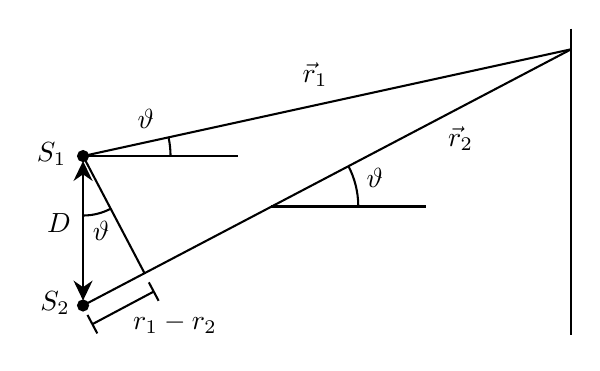
\begin{tikzpicture}[x=0.75pt,y=0.75pt,yscale=-0.9,xscale=0.9]
	%uncomment if require: \path (0,300); %set diagram left start at 0, and has height of 300

	%Shape: Circle [id:dp9911458442903904] 
	\draw  [fill={rgb, 255:red, 0; green, 0; blue, 0 }  ,fill opacity=1 ] (245,149.67) .. controls (245,148.19) and (246.19,147) .. (247.67,147) .. controls (249.14,147) and (250.33,148.19) .. (250.33,149.67) .. controls (250.33,151.14) and (249.14,152.33) .. (247.67,152.33) .. controls (246.19,152.33) and (245,151.14) .. (245,149.67) -- cycle ;
	%Shape: Circle [id:dp9902185672506356] 
	\draw  [fill={rgb, 255:red, 0; green, 0; blue, 0 }  ,fill opacity=1 ] (245,229.67) .. controls (245,228.19) and (246.19,227) .. (247.67,227) .. controls (249.14,227) and (250.33,228.19) .. (250.33,229.67) .. controls (250.33,231.14) and (249.14,232.33) .. (247.67,232.33) .. controls (246.19,232.33) and (245,231.14) .. (245,229.67) -- cycle ;
	%Straight Lines [id:da6057152889101978] 
	\draw    (509,81.5) -- (509,245.5) ;
	%Straight Lines [id:da4873729451655593] 
	\draw    (509,92.5) -- (247.67,229.67) ;
	%Straight Lines [id:da8139723340308482] 
	\draw    (509,92.5) -- (247.67,149.67) ;
	%Straight Lines [id:da30832811432688634] 
	\draw    (330.5,149.67) -- (247.67,149.67) ;
	%Straight Lines [id:da4562670545035852] 
	\draw    (431,176.67) -- (348.17,176.67) ;
	%Shape: Arc [id:dp7854871689199094] 
	\draw  [draw opacity=0] (293.52,140.1) .. controls (294.14,143.07) and (294.47,146.14) .. (294.5,149.29) -- (247.67,149.67) -- cycle ; \draw   (293.52,140.1) .. controls (294.14,143.07) and (294.47,146.14) .. (294.5,149.29) ;
	%Shape: Arc [id:dp12821468762939858] 
	\draw  [draw opacity=0] (389.71,155.02) .. controls (393.03,161.39) and (394.94,168.62) .. (395,176.29) -- (348.17,176.67) -- cycle ; \draw   (389.71,155.02) .. controls (393.03,161.39) and (394.94,168.62) .. (395,176.29) ;
	%Straight Lines [id:da6348505628449739] 
	\draw    (247.67,155.33) -- (247.67,224) ;
	\draw [shift={(247.67,227)}, rotate = 270] [fill={rgb, 255:red, 0; green, 0; blue, 0 }  ][line width=0.08]  [draw opacity=0] (10.72,-5.15) -- (0,0) -- (10.72,5.15) -- (7.12,0) -- cycle    ;
	\draw [shift={(247.67,152.33)}, rotate = 90] [fill={rgb, 255:red, 0; green, 0; blue, 0 }  ][line width=0.08]  [draw opacity=0] (10.72,-5.15) -- (0,0) -- (10.72,5.15) -- (7.12,0) -- cycle    ;
	%Straight Lines [id:da39999949135956214] 
	\draw    (280.5,212.22) -- (247.67,149.67) ;
	%Shape: Arc [id:dp47411815496431053] 
	\draw  [draw opacity=0] (262.44,177.87) .. controls (258.08,180.16) and (253.12,181.47) .. (247.86,181.5) -- (247.67,149.67) -- cycle ; \draw   (262.44,177.87) .. controls (258.08,180.16) and (253.12,181.47) .. (247.86,181.5) ;
	%Straight Lines [id:da17885638933016845] 
	\draw    (285.5,222.22) -- (252.67,239.67) ;
	\draw [shift={(252.67,239.67)}, rotate = 332.02] [color={rgb, 255:red, 0; green, 0; blue, 0 }  ][line width=0.75]    (0,5.59) -- (0,-5.59)   ;
	\draw [shift={(285.5,222.22)}, rotate = 332.02] [color={rgb, 255:red, 0; green, 0; blue, 0 }  ][line width=0.75]    (0,5.59) -- (0,-5.59)   ;

	% Text Node
	\draw (230.83,148.67) node  [font=\normalsize]  {$S_{1}$};
	% Text Node
	\draw (232.67,228.5) node  [font=\normalsize]  {$S_{2}$};
	% Text Node
	\draw (281.33,129.67) node  [font=\normalsize]  {$\vartheta $};
	% Text Node
	\draw (403.83,161.17) node  [font=\normalsize]  {$\vartheta $};
	% Text Node
	\draw (371.83,106.17) node  [font=\normalsize]  {$\vec{r}_{1}$};
	% Text Node
	\draw (449.83,140.17) node  [font=\normalsize]  {$\vec{r}_{2}$};
	% Text Node
	\draw (234.83,185.67) node  [font=\normalsize]  {$D$};
	% Text Node
	\draw (257.33,189.67) node  [font=\normalsize]  {$\vartheta $};
	% Text Node
	\draw (296.83,239.17) node  [font=\normalsize]  {$r_{1} -r_{2}$};

	\end{tikzpicture}
\end{figure}
\FloatBarrier

$I_1$ e $I_2$ in $P$ sarebbero chiaramente diverse, ma se ci concentriamo su una regione sullo schermo abbastanza prossima al centro, per valori di $\vartheta$ quindi non troppo grandi, sostanzialmente le intensità sono uguali se le sorgenti sono identiche.

\begin{align*}
	I(\vartheta) &= 2I_0 [ 1 + \cos (\Delta \Phi)] \\
	&= 2I_0 [ 1 + \cos (\overbrace{kD\sin \vartheta}^{\Delta \Phi})] \tag*{$\frac{1+\cos \alpha}{2}=\cos^2 \left( \frac{\alpha}{2} \right)  $}\\
	&= 4I_0\cos^2 \left( \frac{kD\sin \vartheta}{2} \right)
\end{align*}

I massimi di interferenza si trovano come segue:

\begin{align*}
	\Delta \Phi &= 2\pi m \\
	kD\sin \vartheta &= 2\pi m \\
	\frac{2\pi}{\lambda}D\sin \vartheta &=2\pi m \\
	\Aboxed{\sin \vartheta &=m\frac{\lambda}{D}}
\end{align*}

\section{Inferenza in lamine sottili di materiale dielettrico}

L'interferenza dovuta alla riflessione della luce sulle due superfici di una lamina sottile di una sostanza trasparente è il caso di interferenza più facilmente osservabile nella vita comune. Supponiamo di disporre di una lamina molto sottile di indice di rifrazione $n_2$. Tale lamina è immersa in un altro dielettrico, ad esempio l'aria, di indice $n_1$. Sia $d$ lo spessore della lamina.

\begin{figure}[htpb]
	\centering

	\tikzset{every picture/.style={line width=0.75pt}} %set default line width to 0.75pt        

	\begin{tikzpicture}[x=0.75pt,y=0.75pt,yscale=-1,xscale=1]
	%uncomment if require: \path (0,300); %set diagram left start at 0, and has height of 300

	%Shape: Rectangle [id:dp24401556706323402] 
	\draw   (179,142) -- (503,142) -- (503,170.5) -- (179,170.5) -- cycle ;
	%Straight Lines [id:da6143374172020759] 
	\draw    (313,52.5) -- (313,139) ;
	\draw [shift={(313,142)}, rotate = 270] [fill={rgb, 255:red, 0; green, 0; blue, 0 }  ][line width=0.08]  [draw opacity=0] (10.72,-5.15) -- (0,0) -- (10.72,5.15) -- (7.12,0) -- cycle    ;
	%Straight Lines [id:da4538070003023835] 
	\draw    (333,142) -- (333,167.5) ;
	\draw [shift={(333,170.5)}, rotate = 270] [fill={rgb, 255:red, 0; green, 0; blue, 0 }  ][line width=0.08]  [draw opacity=0] (10.72,-5.15) -- (0,0) -- (10.72,5.15) -- (7.12,0) -- cycle    ;
	%Straight Lines [id:da5117695983840902] 
	\draw    (341,145) -- (341,170.5) ;
	\draw [shift={(341,142)}, rotate = 90] [fill={rgb, 255:red, 0; green, 0; blue, 0 }  ][line width=0.08]  [draw opacity=0] (10.72,-5.15) -- (0,0) -- (10.72,5.15) -- (7.12,0) -- cycle    ;
	%Straight Lines [id:da8396691056997594] 
	\draw    (341,55.5) -- (341,142) ;
	\draw [shift={(341,52.5)}, rotate = 90] [fill={rgb, 255:red, 0; green, 0; blue, 0 }  ][line width=0.08]  [draw opacity=0] (10.72,-5.15) -- (0,0) -- (10.72,5.15) -- (7.12,0) -- cycle    ;
	%Straight Lines [id:da16556866549700122] 
	\draw    (324,55.5) -- (324,142) ;
	\draw [shift={(324,52.5)}, rotate = 90] [fill={rgb, 255:red, 0; green, 0; blue, 0 }  ][line width=0.08]  [draw opacity=0] (10.72,-5.15) -- (0,0) -- (10.72,5.15) -- (7.12,0) -- cycle    ;
	%Straight Lines [id:da5274788703770195] 
	\draw    (323,170.5) -- (323,215.67) ;
	\draw [shift={(323,218.67)}, rotate = 270] [fill={rgb, 255:red, 0; green, 0; blue, 0 }  ][line width=0.08]  [draw opacity=0] (10.72,-5.15) -- (0,0) -- (10.72,5.15) -- (7.12,0) -- cycle    ;

	% Text Node
	\draw (324.67,38.33) node    {$1$};
	% Text Node
	\draw (341.33,38.33) node    {$2$};
	% Text Node
	\draw (200.67,127.33) node    {$n_{1}$};
	% Text Node
	\draw (219.67,154.33) node    {$n_{2}  >n_{1}$};

	\end{tikzpicture}
\end{figure}
\FloatBarrier

Vi è un onda che incide perpendicolarmente. Una parte della luce incidente sulla lamina è riflessa dalla superficie superiore (onda $2$); l'onda trasmessa si propaga nella lamina ed è parzialmente riflessa dalla superficie inferiore. La parte riflessa (onda $1$) riattraversa la lamina e riemerge nel primo mezzo con direzione parallela a quella del primo raggio riflesso. Le due onde giungono all'occhio sfasate: l'onda $2$ per la differenza di cammino ottico $2d$, l'onda $1$ per lo sfasamento di $\pi$ subito alla prima riflessione (dato che $n_1<n_2$). Le due fasi saranno date da:

\[
	\Phi_2 = \pi \qquad \Phi_1 = k\cdot 2d
\]

Le due onde sono sfasate di $\pi$ per quanto detto sull'incidenza normale alla superficie di separazione.
Utilizzando le forme di Fresnel troviamo che:

\[
	\frac{E_r}{E_i} = \frac{n_1-n_2}{n_1+n_2}<0 \qquad \frac{E_r'}{E_i'} = \frac{n_2-n_1}{n_1+n_2}>0
\]

Le due onde sono coerenti, quindi è possibile osservare interferenza fra queste due onde riflesse.

\[
	\Phi_1 = \frac{2\pi n_2}{\lambda}\cdot 2d=\frac{4\pi n_2d}{\lambda}
\]

Calcolando la differenza di fase fra le due onde:

\[
	\Delta \Phi =\Phi_1-\Phi_2 =\frac{4\pi n_2d}{\lambda}  - \pi
\]

Cerchiamo quali sono le condizioni per avere interferenza costruttiva.

\begin{align*}
	\Delta \Phi &= 2\pi m\\
	\frac{4\pi n_2d}{\lambda}  - \pi  &= 2\pi m\\
	\frac{4 n_2d}{\lambda}  - 1  &= 2 m\\
	\frac{4n_2d}{\lambda} &= 2m+1 \\
	\Aboxed{\lambda &= \frac{4n_2d}{2m+1}}
\end{align*}

Questa relazione ci permette di vedere a quale lunghezza d'onda abbiamo interferenza costruttiva. Supponiamo di illuminare la lamina con della luce bianca. La formula ci dice che vedremo la riflessione solo di quelle lunghezze d'onda che obbediscono all'interferenza costruttiva. I colori che si vedono ad esempio riflessi sulle bolle di sapone corrispondono all'interferenza costruttiva della loro superficie. Ci saranno poi altre lunghezze d'onda che daranno interferenza distruttiva e che quindi non vedremo perché si cancellano.

\section{Cenni ai fenomeni diffrattivi}

La diffrazione è una particolare forma di interferenza che appare quando un'onda elettromagnetica incide su un ostacolo o su uno schermo in cui è stata praticata un apertura. Qualitativamente, nello spazio oltre l'ostacolo o l'apertura, le onde si propagano anche lungo direzioni diverse da quella di incidenza e hanno origine differenze di cammino tra onde che si sovrappongono in un dato punto; ecco perché possono avvenire fenomeni di interferenza con conseguente ridistribuzione dell'energia nei punti dello spazio. Gli effetti della diffrazione sono di norma tanto più vistosi quanto più le dimensioni dell'apertura o dell'ostacolo sono vicine al valore della lunghezza d'onda delle onde incidenti. I fenomeni di diffrazione si verificano con tutti i tipi di onde; essi si osservano facilmente nel caso di onde sulla superficie di un liquido e delle onde sonore, aventi lunghezze d'onda prossime alle dimensioni di oggetti molto comuni. Più difficile è l'osservazione nel caso di onde luminose, proprio a causa della piccola lunghezza d'onda. Per capire come si propaghino oltre ad un ostacolo o un foro, sarebbe possibile partire dalle equazioni di Maxwell e risolvere il problema con le condizioni al contorno. Vista la complessità di questo metodo, si utilizza però un approccio più semplice, basato sul \textbf{principio di Huygens-Fresnel}. Esso, che era stato introdotto in forma semi empirica, durante il 19esimo secolo è stato dimostrato in forma rigorosa tramite il teorema di Kirchhoff. Supponiamo di avere un'onda elettromagnetica sinusoidale. Consideriamo un fronte d'onda di essa (la fase è costante in tutti i suoi punti) e suddividiamolo in aree infinitesime. Ciascuna di queste può essere considerata come una sorgente puntiforme di onde sferiche che propagano nello spazio. Il principio afferma che il valore dell'onda in un punto $P$ si può calcolare come sovrapposizione dei campi elettrici prodotti dalle sorgenti puntiformi associate alle aree. Dobbiamo determinare come esprimere ciascuna di queste onde sferiche.

\begin{figure}[htpb]
	\centering

	\tikzset{every picture/.style={line width=0.75pt}} %set default line width to 0.75pt        

	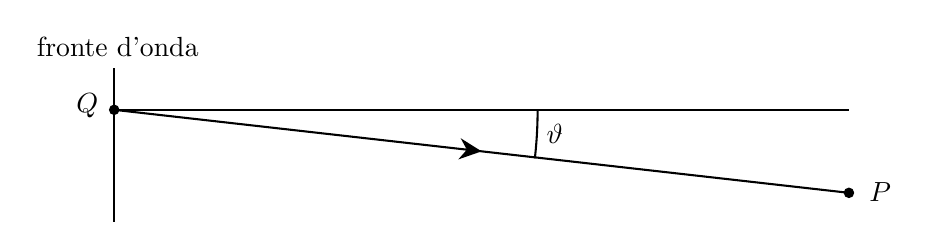
\begin{tikzpicture}[x=0.75pt,y=0.75pt,yscale=-1,xscale=1]
	%uncomment if require: \path (0,300); %set diagram left start at 0, and has height of 300

	%Straight Lines [id:da4386397553414383] 
	\draw    (199,65.5) -- (199,139.5) ;
	%Straight Lines [id:da4550684617529315] 
	\draw    (199,85.5) -- (553,85.5) ;
	%Straight Lines [id:da5825124480043755] 
	\draw    (199,85.5) -- (553,125.5) ;
	\draw [shift={(376,105.5)}, rotate = 186.45] [fill={rgb, 255:red, 0; green, 0; blue, 0 }  ][line width=0.08]  [draw opacity=0] (10.72,-5.15) -- (0,0) -- (10.72,5.15) -- (7.12,0) -- cycle    ;
	%Shape: Arc [id:dp1439929142239722] 
	\draw  [draw opacity=0] (403,85.32) .. controls (403,85.38) and (403,85.44) .. (403,85.5) .. controls (403,93.41) and (402.55,101.21) .. (401.67,108.88) -- (199,85.5) -- cycle ; \draw   (403,85.32) .. controls (403,85.38) and (403,85.44) .. (403,85.5) .. controls (403,93.41) and (402.55,101.21) .. (401.67,108.88) ;
	%Shape: Circle [id:dp40378381740495084] 
	\draw  [fill={rgb, 255:red, 0; green, 0; blue, 0 }  ,fill opacity=1 ] (551,125.5) .. controls (551,124.4) and (551.9,123.5) .. (553,123.5) .. controls (554.1,123.5) and (555,124.4) .. (555,125.5) .. controls (555,126.6) and (554.1,127.5) .. (553,127.5) .. controls (551.9,127.5) and (551,126.6) .. (551,125.5) -- cycle ;
	%Shape: Circle [id:dp7859178245765386] 
	\draw  [fill={rgb, 255:red, 0; green, 0; blue, 0 }  ,fill opacity=1 ] (197,85.5) .. controls (197,84.4) and (197.9,83.5) .. (199,83.5) .. controls (200.1,83.5) and (201,84.4) .. (201,85.5) .. controls (201,86.6) and (200.1,87.5) .. (199,87.5) .. controls (197.9,87.5) and (197,86.6) .. (197,85.5) -- cycle ;

	% Text Node
	\draw (411.33,97) node    {$\vartheta $};
	% Text Node
	\draw (568,125) node    {$P$};
	% Text Node
	\draw (186,83.67) node    {$Q$};
	% Text Node
	\draw (200.67,55) node   [align=left] {fronte d'onda};

	\end{tikzpicture}
\end{figure}
\FloatBarrier

Consideriamo un punto $Q$ del fronte d'onda e tracciamo la congiungente tra il punto $Q$ ed il punto $P$. Introduciamo un versore normale a tale fronte e chiamiamo $\vartheta$ l'angolo che la congiungente forma con esso. Secondo tale principio, l'ampiezza del campo nel punto $P$ prodotto dalla sorgente puntiforme fittizia in $Q$ si ottiene come:

\[
	dE(P)=\frac{E(Q)}{r\lambda}f(\vartheta) dS \qquad f(\vartheta)=\frac{1+\cos \vartheta}{2}
\]

Questa funzione è detta \textbf{funzione di obliquità}. Il principio afferma anche che l'onda secondaria (cioè quella emessa da $Q$) è in anticipo di fase di $\pi/2$ rispetto all'onda principale (ossia l'onda di cui stiamo studiando la propagazione). Calcolando il campo nel punto $P$, sommando le varie onde:

\begin{align*}
	\vec{E} (P)&=\int_{\Sigma}dE(P)\sin \left( kr-\omega t - \frac{\pi}{2} \right)\\
	&=\int_{\Sigma}  \frac{E(Q)}{r\lambda}f(\vartheta) \sin \left( kr-\omega t - \frac{\pi}{2} \right) dS
\end{align*}

Notiamo che:

\begin{itemize}
	\item Per $\vartheta=\pi$ stiamo considerando le onde che si propagano all'indietro, $f(\vartheta)=0$ minimo di $f$.
	\item Per $\vartheta=0$, $f(\vartheta)=1$ massimo di $f$.
\end{itemize}

Possiamo capire come l'integrale sopra calcolato dia maggiore importanza ai contributi che si propagano in avanti ed esclude quelli che tornano indietro.
\textbf{Osservazione.} Avendo a che fare con onde sferiche, non si utilizza l'espressione vettoriale per i campi. La teoria della diffrazione prende il nome anche di teoria scalare.

\section{Diffrazione ad una fenditura rettilinea}

Vediamo cosa accade nel caso di interazione con un ostacolo. Consideriamo l'interazione con una fenditura praticata in uno schermo opaco, di forma rettangolare di altezza $h$, larghezza $d$. Su tale schermo incide un'onda piana elettromagnetica e sinusoidale.

\begin{figure}[htpb]
	\centering

	\tikzset{every picture/.style={line width=0.75pt}} %set default line width to 0.75pt        

	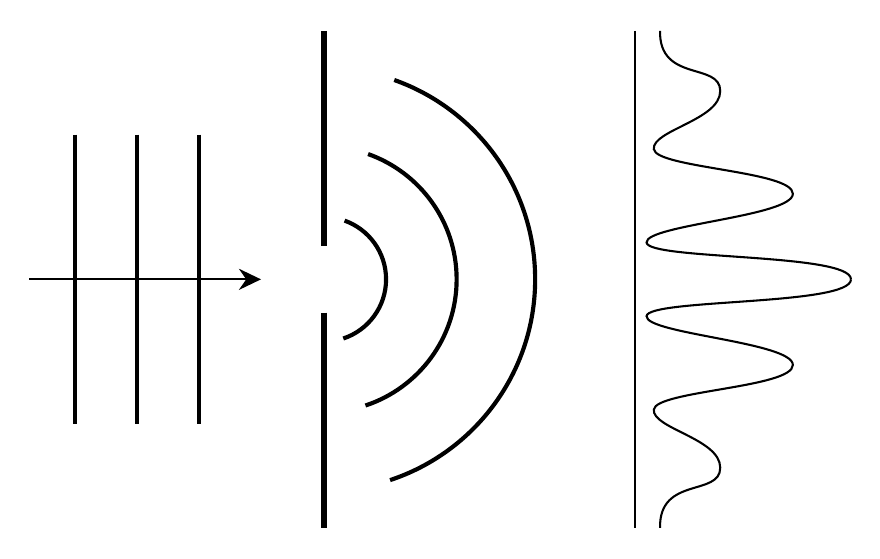
\begin{tikzpicture}[x=0.75pt,y=0.75pt,yscale=-1,xscale=1]
	%uncomment if require: \path (0,300); %set diagram left start at 0, and has height of 300

	%Curve Lines [id:da5914380383052462] 
	\draw    (382.5,36.25) .. controls (382,61.25) and (411.5,51.25) .. (411.5,65.25) .. controls (411.5,79.25) and (378.62,84.15) .. (379.5,93.25) .. controls (380.38,102.35) and (446.5,103.75) .. (446.5,114.75) .. controls (446.5,125.75) and (375.5,129.75) .. (376,138.25) .. controls (376.5,146.75) and (474.5,143.25) .. (474.5,156) ;
	%Curve Lines [id:da04832983911044875] 
	\draw    (382.5,275.75) .. controls (382,250.75) and (411.5,260.75) .. (411.5,246.75) .. controls (411.5,232.75) and (378.62,227.85) .. (379.5,218.75) .. controls (380.38,209.65) and (446.5,208.25) .. (446.5,197.25) .. controls (446.5,186.25) and (375.5,182.25) .. (376,173.75) .. controls (376.5,165.25) and (474.5,168.75) .. (474.5,156) ;
	%Straight Lines [id:da546076973690863] 
	\draw    (370.5,36.25) -- (370.5,275.75) ;
	%Straight Lines [id:da7212551859058829] 
	\draw [line width=2.25]    (220.5,36.25) -- (220.5,140) ;
	%Straight Lines [id:da466265345750674] 
	\draw [line width=2.25]    (220.5,172) -- (220.5,275.75) ;
	%Straight Lines [id:da9852288833275191] 
	\draw [line width=1.5]    (130.5,86.25) -- (130.5,225.75) ;
	%Straight Lines [id:da08948640210316205] 
	\draw [line width=1.5]    (160.5,86.25) -- (160.5,225.75) ;
	%Straight Lines [id:da9783729066556608] 
	\draw [line width=1.5]    (100.5,86.25) -- (100.5,225.75) ;
	%Straight Lines [id:da9867791784292883] 
	\draw [line width=0.75]    (187.25,156) -- (78.33,156) ;
	\draw [shift={(190.25,156)}, rotate = 180] [fill={rgb, 255:red, 0; green, 0; blue, 0 }  ][line width=0.08]  [draw opacity=0] (10.72,-5.15) -- (0,0) -- (10.72,5.15) -- (7.12,0) -- cycle    ;
	%Shape: Arc [id:dp5890001897873898] 
	\draw  [draw opacity=0][line width=1.5]  (230.5,127.71) .. controls (242.15,131.83) and (250.5,142.94) .. (250.5,156) .. controls (250.5,169.28) and (241.87,180.55) .. (229.9,184.5) -- (220.5,156) -- cycle ; \draw  [line width=1.5]  (230.5,127.71) .. controls (242.15,131.83) and (250.5,142.94) .. (250.5,156) .. controls (250.5,169.28) and (241.87,180.55) .. (229.9,184.5) ;
	%Shape: Arc [id:dp3857484668049591] 
	\draw  [draw opacity=0][line width=1.5]  (241.84,95.64) .. controls (266.69,104.43) and (284.5,128.14) .. (284.5,156) .. controls (284.5,184.34) and (266.08,208.38) .. (240.56,216.79) -- (220.5,156) -- cycle ; \draw  [line width=1.5]  (241.84,95.64) .. controls (266.69,104.43) and (284.5,128.14) .. (284.5,156) .. controls (284.5,184.34) and (266.08,208.38) .. (240.56,216.79) ;
	%Shape: Arc [id:dp6477878378582584] 
	\draw  [draw opacity=0][line width=1.5]  (254.45,59.96) .. controls (294,73.95) and (322.33,111.66) .. (322.33,156) .. controls (322.33,201.09) and (293.02,239.34) .. (252.42,252.73) -- (220.5,156) -- cycle ; \draw  [line width=1.5]  (254.45,59.96) .. controls (294,73.95) and (322.33,111.66) .. (322.33,156) .. controls (322.33,201.09) and (293.02,239.34) .. (252.42,252.73) ;

	\end{tikzpicture}
\end{figure}
\FloatBarrier

Assumeremo $h\gg d$.
Nei punti in cui non c'è fenditura l'onda viene assorbita. Possiamo applicare il principio di Huygens-Fresnel per calcolare l'andamento dell'onda oltre la fenditura.
Consideriamo un certo punto $P$ dello schermo. Introduciamo un asse ortogonale ad esso. Individuiamo la posizione di $P$ con un angolo formato dalla congiungente $QP$ con la normale. Suddividiamo la fenditura in tante aree. Essendo essa rettangolare, possiamo immaginare che esse siano strisce di lunghezza $h$ e ampiezza $dx$.

\begin{figure}[htpb]
	\centering

	\tikzset{every picture/.style={line width=0.75pt}} %set default line width to 0.75pt        

	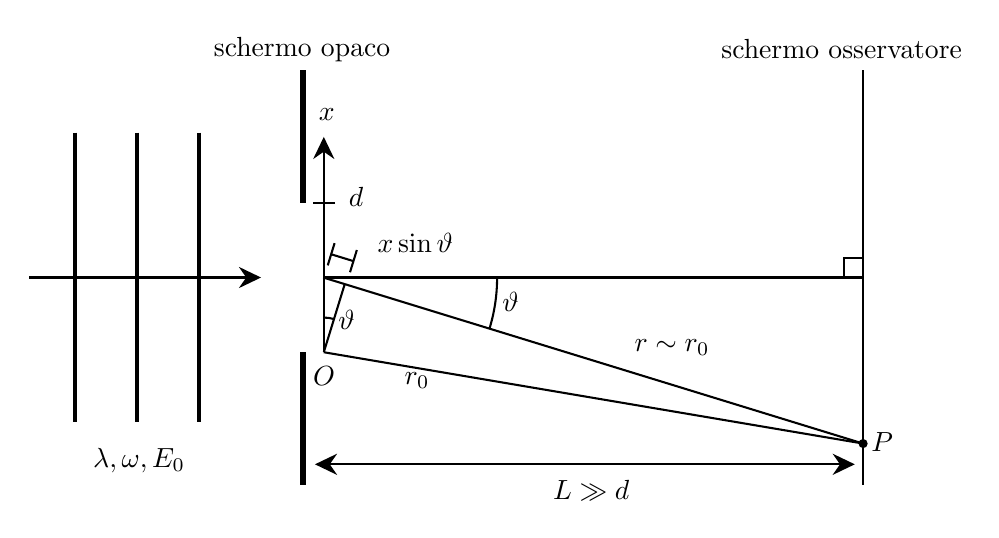
\begin{tikzpicture}[x=0.75pt,y=0.75pt,yscale=-1,xscale=1]
	%uncomment if require: \path (0,300); %set diagram left start at 0, and has height of 300

	%Straight Lines [id:da7994316663783338] 
	\draw    (470.5,46.25) -- (470.5,245.75) ;
	%Straight Lines [id:da3631398435488242] 
	\draw [line width=2.25]    (200.5,46.25) -- (200.5,110) ;
	%Straight Lines [id:da3478792651437992] 
	\draw [line width=2.25]    (200.5,182) -- (200.5,245.75) ;
	%Straight Lines [id:da4931368342341502] 
	\draw [line width=1.5]    (120.5,76.25) -- (120.5,215.75) ;
	%Straight Lines [id:da6396195075323743] 
	\draw [line width=1.5]    (150.5,76.25) -- (150.5,215.75) ;
	%Straight Lines [id:da46727844054075396] 
	\draw [line width=1.5]    (90.5,76.25) -- (90.5,215.75) ;
	%Straight Lines [id:da6344169929086054] 
	\draw [line width=0.75]    (177.25,146) -- (68.33,146) ;
	\draw [shift={(180.25,146)}, rotate = 180] [fill={rgb, 255:red, 0; green, 0; blue, 0 }  ][line width=0.08]  [draw opacity=0] (10.72,-5.15) -- (0,0) -- (10.72,5.15) -- (7.12,0) -- cycle    ;
	%Straight Lines [id:da9436036410898272] 
	\draw    (210.5,81.25) -- (210.5,182) ;
	\draw [shift={(210.5,78.25)}, rotate = 90] [fill={rgb, 255:red, 0; green, 0; blue, 0 }  ][line width=0.08]  [draw opacity=0] (10.72,-5.15) -- (0,0) -- (10.72,5.15) -- (7.12,0) -- cycle    ;
	%Straight Lines [id:da8833480033622181] 
	\draw    (470.33,146) -- (210.25,146) ;
	%Straight Lines [id:da8508207041439235] 
	\draw    (463.33,236) -- (209.25,236) ;
	\draw [shift={(206.25,236)}, rotate = 360] [fill={rgb, 255:red, 0; green, 0; blue, 0 }  ][line width=0.08]  [draw opacity=0] (10.72,-5.15) -- (0,0) -- (10.72,5.15) -- (7.12,0) -- cycle    ;
	\draw [shift={(466.33,236)}, rotate = 180] [fill={rgb, 255:red, 0; green, 0; blue, 0 }  ][line width=0.08]  [draw opacity=0] (10.72,-5.15) -- (0,0) -- (10.72,5.15) -- (7.12,0) -- cycle    ;
	%Straight Lines [id:da6080543816878032] 
	\draw    (216,110) -- (205.5,110) ;
	%Straight Lines [id:da2800689018761018] 
	\draw    (470.33,226) -- (210.25,146) ;
	%Straight Lines [id:da21794098535866158] 
	\draw    (470.33,226) -- (210.5,182) ;
	%Shape: Arc [id:dp7291768055910737] 
	\draw  [draw opacity=0] (294,146.25) .. controls (293.97,154.8) and (292.67,163.06) .. (290.26,170.83) -- (210.25,146) -- cycle ; \draw   (294,146.25) .. controls (293.97,154.8) and (292.67,163.06) .. (290.26,170.83) ;
	%Shape: Circle [id:dp5488133986890094] 
	\draw  [fill={rgb, 255:red, 0; green, 0; blue, 0 }  ,fill opacity=1 ] (468.67,226) .. controls (468.67,225.08) and (469.41,224.33) .. (470.33,224.33) .. controls (471.25,224.33) and (472,225.08) .. (472,226) .. controls (472,226.92) and (471.25,227.67) .. (470.33,227.67) .. controls (469.41,227.67) and (468.67,226.92) .. (468.67,226) -- cycle ;
	%Shape: Square [id:dp46177419755755844] 
	\draw   (461,136.67) -- (470.33,136.67) -- (470.33,146) -- (461,146) -- cycle ;
	%Straight Lines [id:da9124192741007744] 
	\draw    (210.5,182) -- (220.6,149.16) ;
	%Straight Lines [id:da9027137350461123] 
	\draw    (224.78,138.1) -- (214.05,134.8) ;
	\draw [shift={(214.05,134.8)}, rotate = 377.1] [color={rgb, 255:red, 0; green, 0; blue, 0 }  ][line width=0.75]    (0,5.59) -- (0,-5.59)   ;
	\draw [shift={(224.78,138.1)}, rotate = 377.1] [color={rgb, 255:red, 0; green, 0; blue, 0 }  ][line width=0.75]    (0,5.59) -- (0,-5.59)   ;
	%Shape: Arc [id:dp5116988879360505] 
	\draw  [draw opacity=0] (210.56,165.3) .. controls (212.23,165.31) and (213.83,165.56) .. (215.35,166.01) -- (210.5,182) -- cycle ; \draw   (210.56,165.3) .. controls (212.23,165.31) and (213.83,165.56) .. (215.35,166.01) ;

	% Text Node
	\draw (210.67,193.33) node    {$O$};
	% Text Node
	\draw (212,67.33) node    {$x$};
	% Text Node
	\draw (200,36) node   [align=left] {schermo opaco};
	% Text Node
	\draw (460,36) node   [align=left] {schermo osservatore};
	% Text Node
	\draw (226,107.33) node    {$d$};
	% Text Node
	\draw (339.33,248.67) node    {$L\gg d$};
	% Text Node
	\draw (255.5,195.83) node    {$r_{0}$};
	% Text Node
	\draw (378.3,179.63) node    {$r\sim r_{0}$};
	% Text Node
	\draw (121.5,234.33) node    {$\lambda ,\omega ,E_{0}$};
	% Text Node
	\draw (300.5,157.73) node    {$\vartheta $};
	% Text Node
	\draw (479.5,225.33) node    {$P$};
	% Text Node
	\draw (254.6,129.33) node    {$x\sin \vartheta $};
	% Text Node
	\draw (221.5,166.33) node    {$\vartheta $};

	\end{tikzpicture}
\end{figure}
\FloatBarrier

\[
	dS=h\,dx \qquad E(P)=\int_{\text{fenditura}}  \frac{E_0}{r\lambda}f(\vartheta) \sin \left( kr-\omega t - \frac{\pi}{2} \right) h\,dx
\]

Se assumiamo lo schermo molto lontano, sostanzialmente $r$ può essere considerata costante per tutti i punti sulla fenditura.
Possiamo porre poi $\vartheta$ circa pari a zero. Con questa approssimazione il campo in $P$ sarà dato da:

\[
	E(P) \simeq \frac{E_0h}{r_0 \lambda} \int_{\text{fenditura}} \sin \left( kr-\omega t - \frac{\pi}{2} \right) dx
\]

L'onda emessa avrà andamento:

\[
	\sin (kr_0-\omega t -\pi /2 )
\]

Essendo lo schermo molto lontano, $\vec{r}$ e $\vec{r}_0$ possono considerarsi circa paralleli e l'angolo mostrato in figura è di conseguenza circa pari a $\vartheta$. Grazie a questa approssimazione, possiamo esprimere la lunghezza del tratto indicato in figura come: $x\sin \vartheta$ e l'onda emessa dal generico punto $Q$ può essere scritta come:

\[
	\sin (kr_0+kx\sin \vartheta -\pi /2 - \omega t)
\]

Ed $E(P)$ sarà dato da:

\[
	E(P) \simeq \frac{E_0h}{r_0 \lambda} \int_0^d  \sin \left( kr_0 +kx\sin \vartheta  -\omega t - \frac{\pi}{2} \right) dx
\]

Chiamiamo $\varphi_0 $ la quantità:

\[
	\varphi_0 = kr_0  -\omega t - \frac{\pi}{2}
\]

E proseguiamo col calcolo:

\begin{align*}
	E(P) &\simeq \frac{E_0h}{r_0 \lambda} \int_0^d  \sin (kx\sin \vartheta  +\varphi_0) dx \\
	&\simeq \frac{E_0h}{r_0 \lambda} \left[ -\frac{\cos (\varphi_0+kx\sin \vartheta)}{k\sin \vartheta} \right]_0^d \\
	&\simeq \frac{E_0h}{r_0\lambda k\sin \vartheta} [-\cos (kd\sin \vartheta +\varphi_0 ) + \cos \varphi_0 ] \tag*{(1)}\\
	&\simeq \frac{E_0h}{r_0\lambda k \sin \vartheta} \cdot 2 \sin \left( \frac{2\varphi_0+kd\sin \vartheta}{2} \right)  \sin \left( -\frac{kd\sin \vartheta}{2} \right)\\
	&\simeq \frac{E_0h}{r_0\lambda \underbrace{\frac{2\pi}{\lambda}}_k \sin \vartheta} \cdot 2 \sin \left( \frac{2\varphi_0+kd\sin \vartheta}{2} \right)  \sin \left( -\frac{kd\sin \vartheta}{2} \right)\\
	&\simeq \frac{E_0h}{\pi r_0\sin \vartheta}\sin \left( kr_0-\omega t - \frac{\pi}{2} + \frac{kd\sin \vartheta}{2}  \right) \sin \left( -\frac{kd\sin \vartheta}{2} \right)
\end{align*}

Dove nel passaggio $(1)$ abbiamo usato l'identità:

\[
	\cos \alpha -\cos \beta =2\sin \left( \frac{\alpha +\beta}{2} \right) \sin \left( \frac{\alpha -\beta}{2} \right)
\]

Siamo a questo punto interessanti al calcolo dell'intensità media dell'onda:

\begin{align*}
	I_m(P) &= \varepsilon_0 \varepsilon_r vE^2 (P) \\
	&= \varepsilon_0 c E^2 (P) \\
	&= \varepsilon_0 c(E^2)_m \\
	&= \varepsilon_0 c \frac{E_0^2 h^2}{\pi^2 r_0^2 \sin^2 \vartheta} \cdot \frac{1}{2} \cdot \sin^2 \left( \frac{kd\sin \vartheta}{2} \right) \\
	&= \varepsilon_0 c \frac{E_0^2 h^2}{\pi^2 r_0^2 2} \cdot  \frac{\sin^2 \left( \frac{kd\sin \vartheta}{2} \right)}{\frac{k^2 d^2 \sin^2 \vartheta}{4}} \cdot \frac{k^2 d^2}{4} \tag*{$\alpha=\frac{kd\sin \vartheta}{2}$} \\
	&= \frac{E_0^2 h^2 k^2 d^2 \varepsilon_0 c}{8\pi^2 r_0^2} \left( \frac{\sin^2 \alpha}{\alpha^2} \right) \\
	\Aboxed{I_m(P) &= I_0\frac{\sin^2 \alpha}{\alpha^2}}
\end{align*}

Capiamo come sullo schermo osservatore non vedremo l'ombra netta della fenditura ma una striscia centrale più intensa (detta \emph{immagine della fenditura}) e delle frangette laterali che via via decrescono.

\begin{figure}[htpb]
	\centering

	\tikzset{every picture/.style={line width=0.75pt}} %set default line width to 0.75pt        

	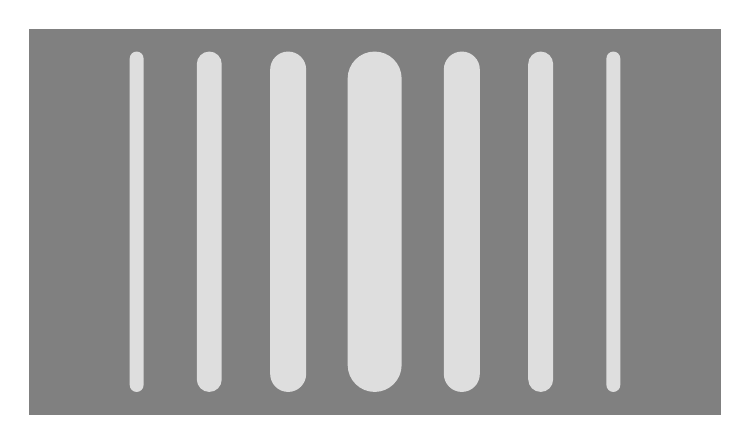
\begin{tikzpicture}[x=0.75pt,y=0.75pt,yscale=-1,xscale=1]
	%uncomment if require: \path (0,300); %set diagram left start at 0, and has height of 300

	%Shape: Rectangle [id:dp4129016214176424] 
	\draw  [draw opacity=0][fill={rgb, 255:red, 128; green, 128; blue, 128 }  ,fill opacity=1 ] (174.33,50.5) -- (507.67,50.5) -- (507.67,236.5) -- (174.33,236.5) -- cycle ;
	%Rounded Rect [id:dp030416714934673017] 
	\draw  [draw opacity=0][fill={rgb, 255:red, 222; green, 222; blue, 222 }  ,fill opacity=1 ] (328,74.5) .. controls (328,67.32) and (333.82,61.5) .. (341,61.5) -- (341,61.5) .. controls (348.18,61.5) and (354,67.32) .. (354,74.5) -- (354,212.5) .. controls (354,219.68) and (348.18,225.5) .. (341,225.5) -- (341,225.5) .. controls (333.82,225.5) and (328,219.68) .. (328,212.5) -- cycle ;
	%Rounded Rect [id:dp3423247111627783] 
	\draw  [draw opacity=0][fill={rgb, 255:red, 222; green, 222; blue, 222 }  ,fill opacity=1 ] (374.33,70.17) .. controls (374.33,65.38) and (378.21,61.5) .. (383,61.5) -- (383,61.5) .. controls (387.79,61.5) and (391.67,65.38) .. (391.67,70.17) -- (391.67,216.83) .. controls (391.67,221.62) and (387.79,225.5) .. (383,225.5) -- (383,225.5) .. controls (378.21,225.5) and (374.33,221.62) .. (374.33,216.83) -- cycle ;
	%Rounded Rect [id:dp3403280424120414] 
	\draw  [draw opacity=0][fill={rgb, 255:red, 222; green, 222; blue, 222 }  ,fill opacity=1 ] (415,67.5) .. controls (415,64.19) and (417.69,61.5) .. (421,61.5) -- (421,61.5) .. controls (424.31,61.5) and (427,64.19) .. (427,67.5) -- (427,219.5) .. controls (427,222.81) and (424.31,225.5) .. (421,225.5) -- (421,225.5) .. controls (417.69,225.5) and (415,222.81) .. (415,219.5) -- cycle ;
	%Rounded Rect [id:dp13891059068839184] 
	\draw  [draw opacity=0][fill={rgb, 255:red, 222; green, 222; blue, 222 }  ,fill opacity=1 ] (452.67,64.83) .. controls (452.67,62.99) and (454.16,61.5) .. (456,61.5) -- (456,61.5) .. controls (457.84,61.5) and (459.33,62.99) .. (459.33,64.83) -- (459.33,222.17) .. controls (459.33,224.01) and (457.84,225.5) .. (456,225.5) -- (456,225.5) .. controls (454.16,225.5) and (452.67,224.01) .. (452.67,222.17) -- cycle ;
	%Rounded Rect [id:dp5743528555322956] 
	\draw  [draw opacity=0][fill={rgb, 255:red, 222; green, 222; blue, 222 }  ,fill opacity=1 ] (308,216.83) .. controls (308,221.62) and (304.12,225.5) .. (299.33,225.5) -- (299.33,225.5) .. controls (294.55,225.5) and (290.67,221.62) .. (290.67,216.83) -- (290.67,70.17) .. controls (290.67,65.38) and (294.55,61.5) .. (299.33,61.5) -- (299.33,61.5) .. controls (304.12,61.5) and (308,65.38) .. (308,70.17) -- cycle ;
	%Rounded Rect [id:dp07505878796940846] 
	\draw  [draw opacity=0][fill={rgb, 255:red, 222; green, 222; blue, 222 }  ,fill opacity=1 ] (267.33,219.5) .. controls (267.33,222.81) and (264.65,225.5) .. (261.33,225.5) -- (261.33,225.5) .. controls (258.02,225.5) and (255.33,222.81) .. (255.33,219.5) -- (255.33,67.5) .. controls (255.33,64.19) and (258.02,61.5) .. (261.33,61.5) -- (261.33,61.5) .. controls (264.65,61.5) and (267.33,64.19) .. (267.33,67.5) -- cycle ;
	%Rounded Rect [id:dp9042984730324282] 
	\draw  [draw opacity=0][fill={rgb, 255:red, 222; green, 222; blue, 222 }  ,fill opacity=1 ] (229.67,222.17) .. controls (229.67,224.01) and (228.17,225.5) .. (226.33,225.5) -- (226.33,225.5) .. controls (224.49,225.5) and (223,224.01) .. (223,222.17) -- (223,64.83) .. controls (223,62.99) and (224.49,61.5) .. (226.33,61.5) -- (226.33,61.5) .. controls (228.17,61.5) and (229.67,62.99) .. (229.67,64.83) -- cycle ;

	\end{tikzpicture}
\end{figure}
\FloatBarrier

I minimi di diffrazione si hanno per $\sin \alpha =0$, in corrispondenza di essi l'intensità dell'onda si annulla.

\[
	\sin \alpha =0 \to \alpha =m\pi \qquad m=0,\pm 1,\pm 2,\ldots
\]

Tra due minimi d'intensità esiste un massimo (detto secondario, a eccezione di quello al centro).

\begin{align*}
	\alpha =\frac{kd\sin \vartheta}{2}= \frac{2\pi d\sin \vartheta}{\lambda 2} = \frac{\pi d\sin \vartheta}{\lambda} &= m \pi \\
	\sin \vartheta &= m\frac{\lambda}{d}
\end{align*}

L'unico caso particolare è quello per $m=0$ invece di avere un minimo abbiamo un massimo.

\section{Diffrazione ad un foro circolare}

Un caso molto interessante è quello della fenditura circolare. La figura di diffrazione, per ragioni di simmetria, consta di un disco luminoso centrale circondato da una serie di corone circolari alternativamente scure e chiare. Queste frange presentano molte analogie con quanto visto nel caso dell'apertura rettilinea, anche se lo studio analitico è più complesso. Se facciamo un grafico dell'intensità della figura di diffrazione in funzione di $\vartheta$, anche in questo caso si ottiene qualcosa di analogo.

\begin{figure}[htpb]
	\centering

	\tikzset{every picture/.style={line width=0.75pt}} %set default line width to 0.75pt        

	
\begin{tikzpicture}[x=0.75pt,y=0.75pt,yscale=-1,xscale=1]
	%uncomment if require: \path (0,300); %set diagram left start at 0, and has height of 300

	%Shape: Rectangle [id:dp5667083945200566] 
	\draw  [draw opacity=0][fill={rgb, 255:red, 128; green, 128; blue, 128 }  ,fill opacity=1 ] (147,68) -- (473,68) -- (473,243) -- (147,243) -- cycle ;
	%Shape: Circle [id:dp6476931658861269] 
	\draw  [draw opacity=0][fill={rgb, 255:red, 222; green, 222; blue, 222 }  ,fill opacity=1 ] (292.33,155.5) .. controls (292.33,145.74) and (300.24,137.83) .. (310,137.83) .. controls (319.76,137.83) and (327.67,145.74) .. (327.67,155.5) .. controls (327.67,165.26) and (319.76,173.17) .. (310,173.17) .. controls (300.24,173.17) and (292.33,165.26) .. (292.33,155.5) -- cycle ;
	%Shape: Circle [id:dp23108609558462168] 
	\draw  [color={rgb, 255:red, 222; green, 222; blue, 222 }  ,draw opacity=1 ][line width=6]  (273,155.5) .. controls (273,135.07) and (289.57,118.5) .. (310,118.5) .. controls (330.43,118.5) and (347,135.07) .. (347,155.5) .. controls (347,175.93) and (330.43,192.5) .. (310,192.5) .. controls (289.57,192.5) and (273,175.93) .. (273,155.5) -- cycle ;
	%Shape: Circle [id:dp08821188808781044] 
	\draw  [color={rgb, 255:red, 222; green, 222; blue, 222 }  ,draw opacity=1 ][line width=4.5]  (252.33,155.5) .. controls (252.33,123.65) and (278.15,97.83) .. (310,97.83) .. controls (341.85,97.83) and (367.67,123.65) .. (367.67,155.5) .. controls (367.67,187.35) and (341.85,213.17) .. (310,213.17) .. controls (278.15,213.17) and (252.33,187.35) .. (252.33,155.5) -- cycle ;
	%Shape: Circle [id:dp6714301698293956] 
	\draw  [color={rgb, 255:red, 222; green, 222; blue, 222 }  ,draw opacity=1 ][line width=2.25]  (234.33,155.5) .. controls (234.33,113.71) and (268.21,79.83) .. (310,79.83) .. controls (351.79,79.83) and (385.67,113.71) .. (385.67,155.5) .. controls (385.67,197.29) and (351.79,231.17) .. (310,231.17) .. controls (268.21,231.17) and (234.33,197.29) .. (234.33,155.5) -- cycle ;

	\end{tikzpicture}
\end{figure}
\FloatBarrier

Si trova in particolare che l'angolo a cui cade il primo minimo di intensità, corrispondente al bordo del disco centrale della figura di diffrazione, è dell'ordine di $1.22\,\lambda/d$. Studiare il caso della fenditura circolare è importante perché tutti gli strumenti ottici (telescopi, microscopi, macchine fotografiche, telecamere ecc...) sono dei sistemi che hanno una limitazione nell'apertura dell'obbiettivo. Quando un onda elettromagnetica incide su uno strumento ottico subisce diffrazione. È ciò che accade se ad esempio osserviamo un oggetto puntiforme con un telescopio. Se il diametro è piccolo, dato che:

\[
	\boxed{\alpha_{\text{min}} = 1.22\,\frac{\lambda}{d}}
\]

la figura sarà molto grande e quindi il telescopio avrà una scarsa risoluzione. Più grande è $d$ più questa figura si stringe.

\section{Limite di risoluzione delle lenti}

Le osservazioni fatte finora sono importanti se vogliamo distinguere due oggetti molto vicini fra di loro e quindi è richiesta una capacità di risoluzione molto elevata.

\begin{figure}[htpb]
	\centering

	\tikzset{every picture/.style={line width=0.75pt}} %set default line width to 0.75pt        

	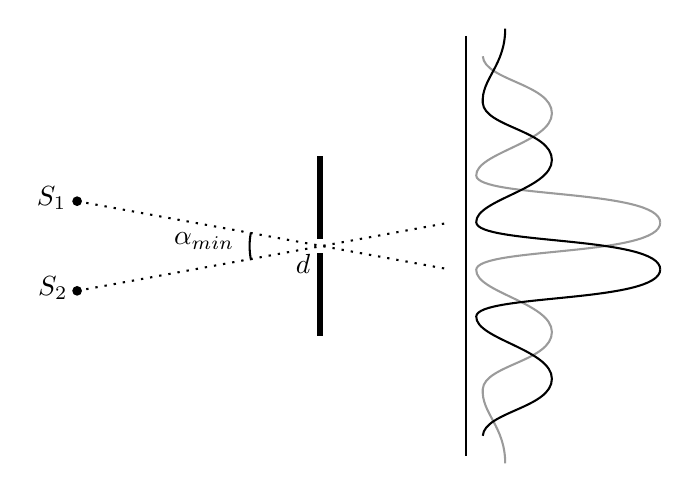
\begin{tikzpicture}[x=0.75pt,y=0.75pt,yscale=-0.9,xscale=0.9]
	%uncomment if require: \path (0,300); %set diagram left start at 0, and has height of 300

	%Curve Lines [id:da38620041188966714] 
	\draw [color={rgb, 255:red, 155; green, 155; blue, 155 }  ,draw opacity=1 ]   (353.5,44.92) .. controls (354.38,57.84) and (390.5,59.82) .. (390.5,75.44) .. controls (390.5,91.06) and (349.5,96.73) .. (350,108.8) .. controls (350.5,120.87) and (448.5,115.9) .. (448.5,134) ;
	%Curve Lines [id:da38887358508281] 
	\draw [color={rgb, 255:red, 155; green, 155; blue, 155 }  ,draw opacity=1 ]   (365.5,262.83) .. controls (365.5,242.96) and (352.62,236) .. (353.5,223.08) .. controls (354.38,210.16) and (390.5,208.18) .. (390.5,192.56) .. controls (390.5,176.94) and (349.5,171.27) .. (350,159.2) .. controls (350.5,147.13) and (448.5,152.1) .. (448.5,134) ;
	%Straight Lines [id:da49895926631976306] 
	\draw  [dash pattern={on 0.84pt off 2.51pt}]  (136.33,170.5) -- (335.5,134) ;
	%Straight Lines [id:da39084005186322335] 
	\draw    (344.5,34) -- (344.5,259) ;
	%Curve Lines [id:da44789670749394483] 
	\draw    (365.5,30.17) .. controls (365.5,50.04) and (352.62,57) .. (353.5,69.92) .. controls (354.38,82.84) and (390.5,84.82) .. (390.5,100.44) .. controls (390.5,116.06) and (349.5,121.73) .. (350,133.8) .. controls (350.5,145.87) and (448.5,140.9) .. (448.5,159) ;
	%Curve Lines [id:da9112796141758652] 
	\draw    (353.5,248.08) .. controls (354.38,235.16) and (390.5,233.18) .. (390.5,217.56) .. controls (390.5,201.94) and (349.5,196.27) .. (350,184.2) .. controls (350.5,172.13) and (448.5,177.1) .. (448.5,159) ;
	%Straight Lines [id:da2237085438594002] 
	\draw [line width=2.25]    (266.33,150.5) -- (266.33,194.67) ;
	%Straight Lines [id:da604548386071253] 
	\draw [line width=2.25]    (266.33,98.33) -- (266.33,142.5) ;
	%Straight Lines [id:da1980329329861159] 
	\draw  [dash pattern={on 0.84pt off 2.51pt}]  (136.33,122.5) -- (335.5,159) ;
	%Shape: Circle [id:dp616090689309877] 
	\draw  [fill={rgb, 255:red, 0; green, 0; blue, 0 }  ,fill opacity=1 ] (134.33,122.5) .. controls (134.33,121.4) and (135.23,120.5) .. (136.33,120.5) .. controls (137.44,120.5) and (138.33,121.4) .. (138.33,122.5) .. controls (138.33,123.6) and (137.44,124.5) .. (136.33,124.5) .. controls (135.23,124.5) and (134.33,123.6) .. (134.33,122.5) -- cycle ;
	%Shape: Circle [id:dp11252939339196733] 
	\draw  [fill={rgb, 255:red, 0; green, 0; blue, 0 }  ,fill opacity=1 ] (134.33,170.5) .. controls (134.33,169.4) and (135.23,168.5) .. (136.33,168.5) .. controls (137.44,168.5) and (138.33,169.4) .. (138.33,170.5) .. controls (138.33,171.6) and (137.44,172.5) .. (136.33,172.5) .. controls (135.23,172.5) and (134.33,171.6) .. (134.33,170.5) -- cycle ;
	%Shape: Arc [id:dp8493492791386488] 
	\draw  [draw opacity=0] (229.43,154.09) .. controls (228.93,151.64) and (228.67,149.1) .. (228.67,146.5) .. controls (228.67,144.05) and (228.9,141.65) .. (229.35,139.32) -- (266.33,146.5) -- cycle ; \draw   (229.43,154.09) .. controls (228.93,151.64) and (228.67,149.1) .. (228.67,146.5) .. controls (228.67,144.05) and (228.9,141.65) .. (229.35,139.32) ;

	% Text Node
	\draw (122.67,121) node    {$S_{1}$};
	% Text Node
	\draw (123.33,169) node    {$S_{2}$};
	% Text Node
	\draw (257.33,156.33) node    {$d$};
	% Text Node
	\draw (204.33,143.83) node    {$\alpha _{min}$};

	\end{tikzpicture}
\end{figure}
\FloatBarrier

Supponiamo di avere due stelle che vogliamo osservare con il telescopio. Esse emettono delle onde piane che arrivano fino a noi. Immaginiamo di rappresentare l'apertura dello strumento con una fenditura circolare. Poniamo che le direzioni di propagazione formino un certo angolo $\alpha$. Sullo schermo appariranno due figure differenti e finché $\alpha \gg\alpha_{min} $, le distinguiamo nettamente. In caso contrario esse si sovrappongono. Esiste un criterio per stabilire qual è la minima distanza angolare alla quale i due oggetti si devono trovare che prende il nome di \textbf{criterio di Rayleigh}. Tale criterio afferma che \emph{siamo in grado distinguere due figure di diffrazione fintanto che la distanza fra di esse è maggiore o uguale a una distanza minima che corrisponde al caso in cui il picco di una delle due figure coincide con il primo minimo dell'altra figura di diffrazione}. Quando la distanza a cui le due figure sono poste è proprio pari a questa distanza minima, si dice che le onde sono \emph{appena risolte}.

\[
	\alpha_{\text{min}} = 1.22\,\frac{\lambda}{d}
\]

Maggiore è il diametro del telescopio, più piccolo sarà l'angolo $\alpha$-minimo a cui riesco a distinguere con risolutezza le stelle. Lavorando nel campo dell'astronomia ottica, quindi osservando la luce, è sufficiente che i telescopi siano del diametro di alcuni metri. Lavorando nel campo della radio astronomia la situazione è differente. Le onde radio hanno $\lambda$ molto maggiore di quella della luce. Per una buona capacità di risoluzione abbiamo bisogno di diametri enormi. I radio telescopi infatti sono parabole gigantesche.

\section{Reticolo di diffrazione}

Invece di avere la singola fenditura potremmo avere fenditure multiple. Il caso più semplice è quello in cui abbiamo due fenditure rettangolari uguali e parallele.

\begin{figure}[htpb]
	\centering

	\tikzset{every picture/.style={line width=0.75pt}} %set default line width to 0.75pt        

	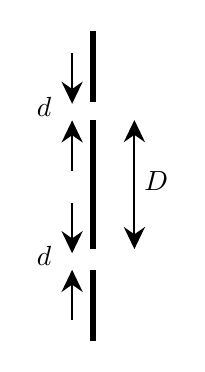
\begin{tikzpicture}[x=0.75pt,y=0.75pt,yscale=-1,xscale=1]
	%uncomment if require: \path (0,300); %set diagram left start at 0, and has height of 300

	%Straight Lines [id:da9982051154678055] 
	\draw [line width=2.25]    (286.33,170.5) -- (286.33,204.67) ;
	%Straight Lines [id:da30716518689549455] 
	\draw [line width=2.25]    (286.33,98.33) -- (286.33,160.5) ;
	%Straight Lines [id:da921180189443459] 
	\draw [line width=2.25]    (286.33,55.33) -- (286.33,89.5) ;
	%Straight Lines [id:da7811689716718062] 
	\draw [line width=0.75]    (276.33,173.5) -- (276.33,194.75) ;
	\draw [shift={(276.33,170.5)}, rotate = 90] [fill={rgb, 255:red, 0; green, 0; blue, 0 }  ][line width=0.08]  [draw opacity=0] (10.72,-5.15) -- (0,0) -- (10.72,5.15) -- (7.12,0) -- cycle    ;
	%Straight Lines [id:da48287849255629745] 
	\draw [line width=0.75]    (276.33,138.25) -- (276.33,159.5) ;
	\draw [shift={(276.33,162.5)}, rotate = 270] [fill={rgb, 255:red, 0; green, 0; blue, 0 }  ][line width=0.08]  [draw opacity=0] (10.72,-5.15) -- (0,0) -- (10.72,5.15) -- (7.12,0) -- cycle    ;
	%Straight Lines [id:da02614628480081649] 
	\draw [line width=0.75]    (276.33,101.5) -- (276.33,122.75) ;
	\draw [shift={(276.33,98.5)}, rotate = 90] [fill={rgb, 255:red, 0; green, 0; blue, 0 }  ][line width=0.08]  [draw opacity=0] (10.72,-5.15) -- (0,0) -- (10.72,5.15) -- (7.12,0) -- cycle    ;
	%Straight Lines [id:da15297787750244418] 
	\draw [line width=0.75]    (276.33,66.25) -- (276.33,87.5) ;
	\draw [shift={(276.33,90.5)}, rotate = 270] [fill={rgb, 255:red, 0; green, 0; blue, 0 }  ][line width=0.08]  [draw opacity=0] (10.72,-5.15) -- (0,0) -- (10.72,5.15) -- (7.12,0) -- cycle    ;
	%Straight Lines [id:da6444856828113377] 
	\draw [line width=0.75]    (306.33,101.33) -- (306.33,157.5) ;
	\draw [shift={(306.33,160.5)}, rotate = 270] [fill={rgb, 255:red, 0; green, 0; blue, 0 }  ][line width=0.08]  [draw opacity=0] (10.72,-5.15) -- (0,0) -- (10.72,5.15) -- (7.12,0) -- cycle    ;
	\draw [shift={(306.33,98.33)}, rotate = 90] [fill={rgb, 255:red, 0; green, 0; blue, 0 }  ][line width=0.08]  [draw opacity=0] (10.72,-5.15) -- (0,0) -- (10.72,5.15) -- (7.12,0) -- cycle    ;

	% Text Node
	\draw (262.83,163.83) node    {$d$};
	% Text Node
	\draw (262.83,91.83) node    {$d$};
	% Text Node
	\draw (316.83,127.83) node    {$D$};

	\end{tikzpicture}
\end{figure}
\FloatBarrier

Si avranno due figure di diffrazione che provengono dalla stessa onda incidente. Siccome si tratta di un onda monocromatica piana, possiamo interpretare la situazione come se avessimo due sorgenti coerenti di onde elettromagnetiche. Abbiamo visto che in presenza di sorgenti coerenti otteniamo un'interferenza. Si ha dunque una combinazione dei due fenomeni.
L'andamento che osserveremo sarà una funzione di interferenza contenuta nell'inviluppo dato dal fenomeno di diffrazione.

\begin{figure}[htpb]
	\centering

	\tikzset{every picture/.style={line width=0.75pt}} %set default line width to 0.75pt        

	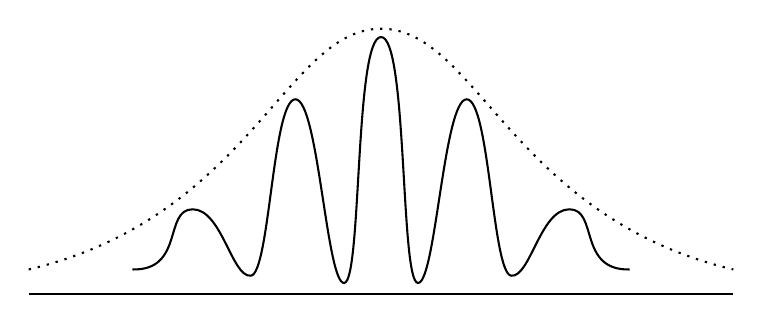
\begin{tikzpicture}[x=0.75pt,y=0.75pt,yscale=-1,xscale=1]
	%uncomment if require: \path (0,300); %set diagram left start at 0, and has height of 300

	%Curve Lines [id:da4430232758282888] 
	\draw    (162.75,196) .. controls (187.75,196.5) and (177.75,167) .. (191.75,167) .. controls (205.75,167) and (210.65,199.88) .. (219.75,199) .. controls (228.85,198.12) and (230.25,114) .. (241.25,114) .. controls (252.25,114) and (256.25,203) .. (264.75,202.5) .. controls (273.25,202) and (269.75,84) .. (282.5,84) ;
	%Curve Lines [id:da3958706293037202] 
	\draw    (402.25,196) .. controls (377.25,196.5) and (387.25,167) .. (373.25,167) .. controls (359.25,167) and (354.35,199.88) .. (345.25,199) .. controls (336.15,198.12) and (334.75,114) .. (323.75,114) .. controls (312.75,114) and (308.75,203) .. (300.25,202.5) .. controls (291.75,202) and (295.25,84) .. (282.5,84) ;
	%Straight Lines [id:da5381577750567956] 
	\draw    (112.75,208) -- (452.25,208) ;
	%Curve Lines [id:da9555907596763293] 
	\draw  [dash pattern={on 0.84pt off 2.51pt}]  (112.75,196) .. controls (219.67,170.67) and (236.67,80) .. (282.5,80) .. controls (328.33,80) and (345.67,170.67) .. (452.25,196) ;

	\end{tikzpicture}
\end{figure}
\FloatBarrier

In termini quantitativi, se introduciamo le quantità $\alpha$ (vista in precedenza) e $\beta$ come:

\[
	\alpha = \frac{kd\sin \vartheta}{2} \qquad \beta =\frac{kD\sin \vartheta}{2}
\]

La figura di interferenza la possiamo scrivere come:

\[
	I = 4I_0\frac{\sin^2 \alpha}{\alpha^2}\cos^2 \beta
\]

Invece di considerare solo due fenditure si può immaginare di considerarne un numero molto grande. Uno schermo in cui ho praticato un numero $N$ molto elevato di fenditure tutte uguali ed equi spaziate prende il nome di \textbf{reticolo di diffrazione}. Osservando quello che accade all'intensità a grande distanza otterremo una funzione con inviluppo dato dalla figura di diffrazione.

Questa volta però avremo dei picchi di interferenza molto più stretti separati da delle oscillazioni molto più piccole.

\begin{figure}[htpb]
	\centering

	\tikzset{every picture/.style={line width=0.75pt}} %set default line width to 0.75pt        

	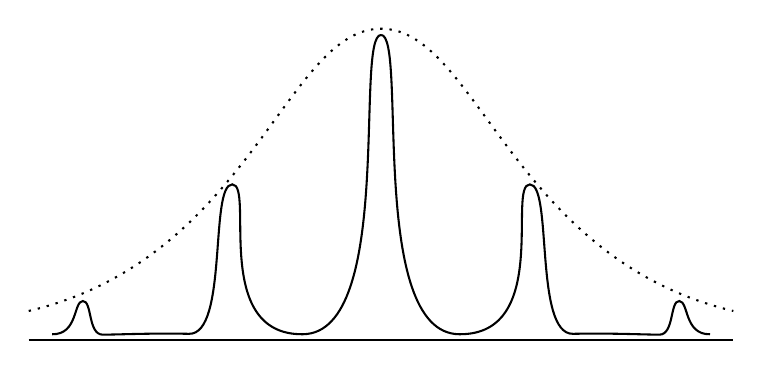
\begin{tikzpicture}[x=0.75pt,y=0.75pt,yscale=-1,xscale=1]
	%uncomment if require: \path (0,300); %set diagram left start at 0, and has height of 300

	%Curve Lines [id:da2879964292305275] 
	\draw    (461,225.2) .. controls (448.5,225.45) and (450.78,209.41) .. (446.2,209.2) .. controls (441.63,208.99) and (443.8,225.4) .. (436.6,225.4) .. controls (429.4,225.4) and (413.8,224.6) .. (395,225) .. controls (376.2,225.4) and (385.2,153) .. (374.2,153) .. controls (363.2,153) and (384.6,225.6) .. (340.2,225.2) .. controls (295.8,224.8) and (315.25,81) .. (302.5,81) ;
	%Straight Lines [id:da5771587807011713] 
	\draw    (132.75,228) -- (472.25,228) ;
	%Curve Lines [id:da6999062790272035] 
	\draw  [dash pattern={on 0.84pt off 2.51pt}]  (132.75,214) .. controls (239.67,188.67) and (256.67,78) .. (302.5,78) .. controls (348.33,78) and (365.67,188.67) .. (472.25,214) ;
	%Curve Lines [id:da02489589483366328] 
	\draw    (144,225.2) .. controls (156.5,225.45) and (154.22,209.41) .. (158.8,209.2) .. controls (163.38,208.99) and (161.2,225.4) .. (168.4,225.4) .. controls (175.6,225.4) and (191.2,224.6) .. (210,225) .. controls (228.8,225.4) and (219.8,153) .. (230.8,153) .. controls (241.8,153) and (220.4,225.6) .. (264.8,225.2) .. controls (309.2,224.8) and (289.75,81) .. (302.5,81) ;

	\end{tikzpicture}
\end{figure}
\FloatBarrier

Invece di osservare un andamento di tipo sinusoidale osserveremo picchi di intensità molto elevata molto separati fra di loro. In tal caso si può dimostrare che l'intensità è data da:

\[
	\boxed{I=I_0\,\frac{\sin^2 \alpha}{\alpha^2}\,\frac{\sin^2 (N\beta)}{\sin^2 \beta}}
\]

Si verifica che per $\vartheta=0 \implies I=N^2 I_0 $, dove $I_0$ è l'intensità massima della figura di diffrazione della singola fenditura.
Se illuminiamo il reticolo di diffrazione con della luce policromatica, ad esempio la luce bianca, per ciascun colore la posizione del picco cambierà. Quest'oggetto funziona come un'analizzatore di schermi, ci consente di separare fra di loro i vari colori perché li vediamo apparire in posizioni diverse.

Il reticolo di diffrazione è la novità che ha consentito di cominciare a studiare in modo dettagliato le proprietà della materia permettendone un'\emph{analisi spettroscopica}. Esso analizza i colori presenti in un fascio di luce monocromatica. Un esempio di reticolo di diffrazione è il \emph{compact disc} (anche se funziona in modo leggermente differente). La sua superficie è infatti costituita da tanti solchi che quando vengono illuminati dall'onda elettromagnetica si comportano un po' come queste fenditure.